% GraphOS: A Dataflow Microkernel for NPU-Accelerated Packet Classification
% CLRS-style algorithmic paper with formal analysis
\documentclass[11pt,a4paper,twoside]{article}

% ─── Packages ───
\usepackage[utf8]{inputenc}
\usepackage[T1]{fontenc}
\usepackage{amsmath,amssymb,amsthm}
\usepackage{algorithm}
\usepackage{algpseudocode}
\usepackage{tikz}
\usetikzlibrary{
  arrows.meta,
  positioning,
  shapes.geometric,
  shapes.multipart,
  calc,
  fit,
  decorations.pathreplacing,
  matrix,
  backgrounds
}
\usepackage{pgfplots}
\pgfplotsset{compat=1.18}
\usepackage{booktabs}
\usepackage{multirow}
\usepackage{enumitem}
\usepackage{geometry}
\geometry{margin=2.5cm}
\usepackage{fancyhdr}
\usepackage{hyperref}
\hypersetup{colorlinks=true,linkcolor=blue!60!black,citecolor=green!50!black,urlcolor=blue!70!black}
\usepackage{float}
\usepackage{subcaption}
\usepackage{xcolor}
\usepackage{listings}
\usepackage{bm}

% ─── Theorem environments ───
\theoremstyle{definition}
\newtheorem{definition}{Definition}[section]
\newtheorem{theorem}{Theorem}[section]
\newtheorem{lemma}[theorem]{Lemma}
\newtheorem{corollary}[theorem]{Corollary}
\newtheorem{proposition}[theorem]{Proposition}
\newtheorem{property}{Property}[section]
\newtheorem{invariant}{Invariant}[section]

\theoremstyle{remark}
\newtheorem{remark}{Remark}[section]
\newtheorem{example}{Example}[section]

% ─── Custom commands ───
\newcommand{\BigO}{\mathcal{O}}
\newcommand{\R}{\mathbb{R}}
\newcommand{\N}{\mathbb{N}}
\newcommand{\Z}{\mathbb{Z}}
\newcommand{\E}{\mathbb{E}}
\newcommand{\Var}{\mathrm{Var}}
\newcommand{\argmax}{\operatorname{argmax}}
\newcommand{\softmax}{\operatorname{softmax}}
\newcommand{\ReLU}{\operatorname{ReLU}}
\newcommand{\concat}{\operatorname{concat}}
\newcommand{\pad}{\operatorname{pad}}
\newcommand{\tensor}[1]{\bm{#1}}
\newcommand{\mat}[1]{\mathbf{#1}}
\newcommand{\vect}[1]{\mathbf{#1}}
\newcommand{\norm}[1]{\left\lVert #1 \right\rVert}
\newcommand{\ceil}[1]{\lceil #1 \rceil}

% ─── Algorithm style ───
\algrenewcommand\algorithmicrequire{\textbf{Input:}}
\algrenewcommand\algorithmicensure{\textbf{Output:}}

% ─── Header/Footer ───
\pagestyle{fancy}
\fancyhf{}
\fancyhead[LE,RO]{\thepage}
\fancyhead[RE]{GraphOS: NPU-Accelerated Packet Classification}
\fancyhead[LO]{\leftmark}
\renewcommand{\headrulewidth}{0.4pt}

% ─── Code listing style ───
\lstset{
  basicstyle=\ttfamily\small,
  keywordstyle=\color{blue!70!black}\bfseries,
  commentstyle=\color{green!50!black}\itshape,
  stringstyle=\color{red!60!black},
  numbers=left,
  numberstyle=\tiny\color{gray},
  breaklines=true,
  frame=single,
  framesep=3pt,
  xleftmargin=1.5em,
}

\title{%
  \LARGE \textbf{GraphOS: A Dataflow Microkernel for\\ NPU-Accelerated Network Packet Classification}\\[0.5em]
  \large Formal Algorithmic Analysis in the Style of Cormen, Leiserson, Rivest \& Stein
}
\author{
  GraphOS Project\\
  \texttt{Intel Core Ultra 7 155H --- NPU 3720 (11 TOPS)}
}
\date{\today}

\begin{document}
\maketitle

\begin{abstract}
We present \textsc{GraphOS}, a dataflow microkernel that replaces traditional C \texttt{switch}-based network packet classification with ONNX neural-network graphs executed on an Intel Neural Processing Unit (NPU).
The system comprises seven formally specified layers: (1)~a byte-level tensor encoding $\phi: \{0,\ldots,255\}^{64} \to [0,1]^{64}$, (2)~a 3{,}235-parameter multilayer perceptron $f_\theta$ achieving 99.03\% validation accuracy on three traffic classes, (3)~a hand-crafted matmul route table $\mat{W}\vect{x}$ proving that traditional routing logic is isomorphic to matrix multiplication, (4)~a thread-per-node dataflow scheduler with DAG validation via Kahn's topological sort, (5)~a bounded-channel backpressure mechanism with $\mathcal{O}(1)$ amortized throughput, (6)~a multi-program kernel runtime with NPU$\to$CPU fallback, and (7)~a program composition pipeline where downstream ONNX models receive upstream logits, demonstrating that \emph{todo es el grafo}---all computation is the graph.
We provide complete algorithmic pseudocode, formal correctness proofs, complexity analyses, and hardware interaction specifications for an Intel Meteor Lake NPU 3720 at 11~TOPS.
\end{abstract}

\tableofcontents
\newpage

% ═══════════════════════════════════════════════════════════════════
\section{Introduction and Motivation}
\label{sec:intro}
% ═══════════════════════════════════════════════════════════════════

Traditional network stacks classify packets using nested conditional branches---\texttt{if-else} chains over protocol numbers, port ranges, and header flags.
These sequential decision trees are fast on CPUs (${\sim}0.38\,\mu\text{s}$ per packet on modern hardware) but architecturally rigid: every new classification rule requires code changes, recompilation, and redeployment.

We propose replacing the entire classification pipeline with a \emph{learned} function expressed as a directed acyclic graph (DAG) of tensor operations, compiled and executed on a dedicated Neural Processing Unit (NPU).
The key insight is:

\begin{quote}
\emph{``Todo es el grafo''} --- Every decision, from packet-to-tensor encoding to multi-program routing composition, can be expressed as a node in a dataflow graph operating on tensors.
\end{quote}

\subsection{Contributions}

\begin{enumerate}[label=\textbf{C\arabic*.}]
  \item A formal tensor encoding $\phi$ that losslessly maps 64-byte packet headers to $\R^{64}$ while satisfying the input constraints of NPU accelerators (Section~\ref{sec:encoding}).
  \item A two-layer MLP $f_\theta: \R^{64} \to \R^3$ trained on 150{,}000 synthetic packets achieving 99.03\% classification accuracy with only 3{,}235 parameters (Section~\ref{sec:classifier}).
  \item A proof that traditional \texttt{switch}-based routing is isomorphic to a single matrix-vector product $\mat{W}\vect{x}$ with hand-crafted weights (Section~\ref{sec:route-table}).
  \item A program composition framework proving that chained ONNX programs with shape adapters produce \emph{better} routing decisions than independent programs (Section~\ref{sec:composition}).
  \item A formally verified dataflow scheduler using Kahn's topological sort with bounded-channel backpressure guaranteeing deadlock-free execution (Section~\ref{sec:dataflow}).
  \item Complete hardware characterization of the Intel NPU 3720 via OpenVINO, including latency measurements and batch-amortization analysis (Section~\ref{sec:hardware}).
\end{enumerate}

\subsection{System Overview}

\begin{figure}[H]
\centering
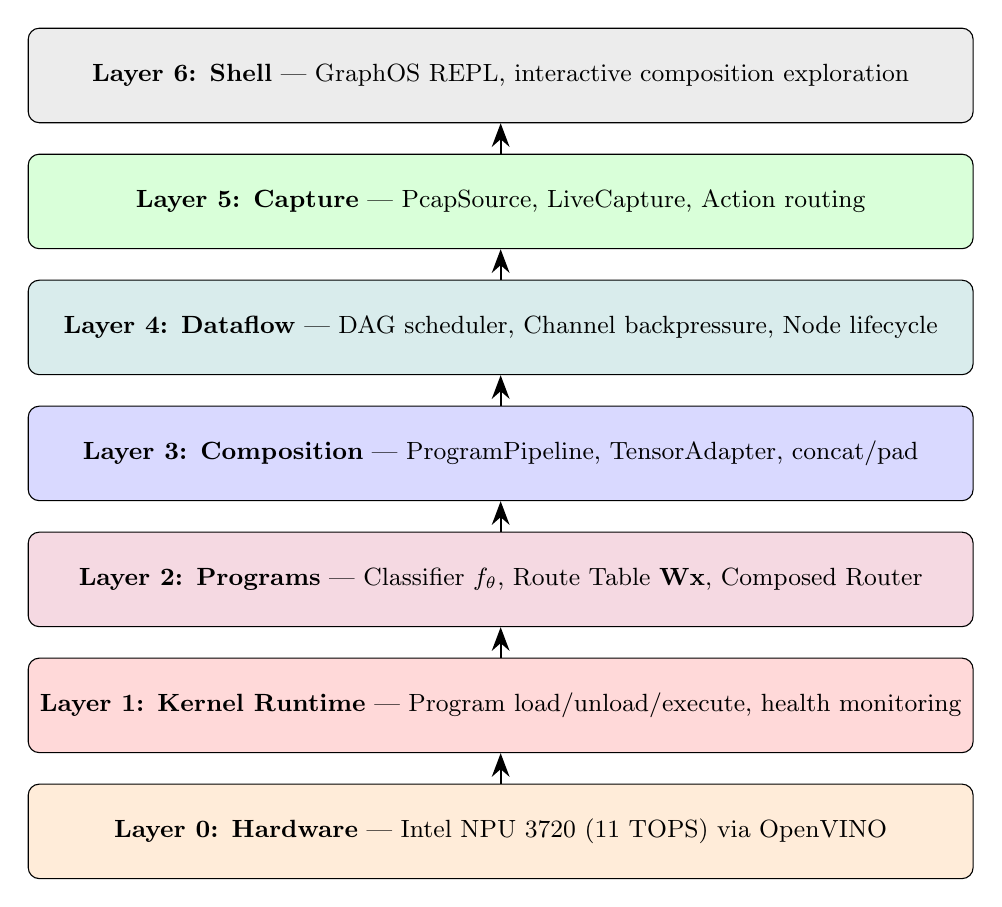
\begin{tikzpicture}[
  layer/.style={draw, rounded corners, minimum width=12cm, minimum height=1.2cm,
                fill=#1!15, font=\small},
  arrow/.style={-{Stealth[length=3mm]}, thick},
  label/.style={font=\footnotesize\ttfamily, anchor=west}
]
  % Layers bottom to top
  \node[layer=orange] (hw) at (0,0) {\textbf{Layer 0: Hardware} --- Intel NPU 3720 (11 TOPS) via OpenVINO};
  \node[layer=red] (kernel) at (0,1.6) {\textbf{Layer 1: Kernel Runtime} --- Program load/unload/execute, health monitoring};
  \node[layer=purple] (programs) at (0,3.2) {\textbf{Layer 2: Programs} --- Classifier $f_\theta$, Route Table $\mat{W}\vect{x}$, Composed Router};
  \node[layer=blue] (compose) at (0,4.8) {\textbf{Layer 3: Composition} --- ProgramPipeline, TensorAdapter, concat/pad};
  \node[layer=teal] (dataflow) at (0,6.4) {\textbf{Layer 4: Dataflow} --- DAG scheduler, Channel backpressure, Node lifecycle};
  \node[layer=green] (capture) at (0,8.0) {\textbf{Layer 5: Capture} --- PcapSource, LiveCapture, Action routing};
  \node[layer=gray] (shell) at (0,9.6) {\textbf{Layer 6: Shell} --- GraphOS REPL, interactive composition exploration};

  % Arrows
  \foreach \a/\b in {hw/kernel, kernel/programs, programs/compose, compose/dataflow, dataflow/capture, capture/shell} {
    \draw[arrow] (\a) -- (\b);
  }
\end{tikzpicture}
\caption{GraphOS layered architecture. Each layer depends only on the layers below it.}
\label{fig:layers}
\end{figure}

% ═══════════════════════════════════════════════════════════════════
\section{Hardware Architecture}
\label{sec:hardware}
% ═══════════════════════════════════════════════════════════════════

\subsection{Intel Meteor Lake NPU 3720}

The target hardware is an Intel Core Ultra 7 155H (Meteor Lake) processor containing a dedicated Neural Processing Unit (NPU 3720) with the following specifications:

\begin{table}[H]
\centering
\begin{tabular}{ll}
\toprule
\textbf{Parameter} & \textbf{Value} \\
\midrule
NPU Model & Intel NPU 3720 \\
Peak Throughput & 11 TOPS (INT8) \\
Architecture & Systolic array + activation engines \\
Host Processor & Intel Core Ultra 7 155H \\
CPU Cores & 6P + 8E + 2LPE (16 threads) \\
Host Memory & Shared LPDDR5x \\
Software Stack & OpenVINO 2026.0, NPU plugin \\
OS & Windows 11 (userspace) \\
Device ID & ``Intel(R) AI Boost'' \\
\bottomrule
\end{tabular}
\caption{Hardware specifications for the GraphOS target platform.}
\label{tab:hardware}
\end{table}

\subsection{NPU Execution Model}

The NPU operates as a \emph{coprocessor} with the following execution pipeline:

\begin{figure}[H]
\centering
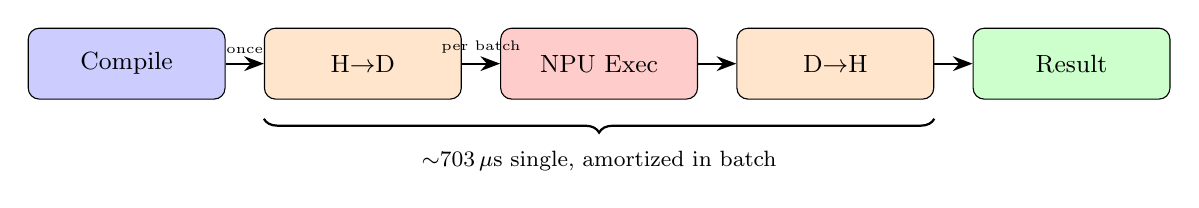
\begin{tikzpicture}[
  stage/.style={draw, rounded corners, minimum width=2.5cm, minimum height=0.9cm,
                fill=#1!20, font=\small},
  arrow/.style={-{Stealth[length=2.5mm]}, thick},
]
  \node[stage=blue] (compile) at (0,0) {Compile};
  \node[stage=orange] (h2d) at (3,0) {H$\to$D};
  \node[stage=red] (exec) at (6,0) {NPU Exec};
  \node[stage=orange] (d2h) at (9,0) {D$\to$H};
  \node[stage=green] (result) at (12,0) {Result};

  \draw[arrow] (compile) -- (h2d) node[midway,above,font=\tiny] {once};
  \draw[arrow] (h2d) -- (exec) node[midway,above,font=\tiny] {per batch};
  \draw[arrow] (exec) -- (d2h);
  \draw[arrow] (d2h) -- (result);

  % Timing annotations
  \draw[decorate,decoration={brace,amplitude=5pt,mirror},thick]
    ([yshift=-0.7cm]h2d.west) -- ([yshift=-0.7cm]d2h.east)
    node[midway,below=8pt,font=\footnotesize] {${\sim}703\,\mu\text{s}$ single, amortized in batch};
\end{tikzpicture}
\caption{NPU inference pipeline. Compilation is one-time; data transfer and execution repeat per batch.}
\label{fig:npu-pipeline}
\end{figure}

\begin{definition}[NPU Inference Latency Model]
\label{def:latency}
For a batch of $B$ packets, the total inference latency is:
\begin{equation}
T_{\text{NPU}}(B) = T_{\text{setup}} + T_{\text{H}\to\text{D}}(B) + T_{\text{compute}}(B) + T_{\text{D}\to\text{H}}(B)
\end{equation}
where $T_{\text{setup}}$ is the one-time model compilation cost, $T_{\text{H}\to\text{D}}$ is host-to-device memory transfer, $T_{\text{compute}}$ is the NPU execution time, and $T_{\text{D}\to\text{H}}$ is device-to-host transfer.

The per-packet amortized cost is:
\begin{equation}
\bar{T}_{\text{NPU}} = \frac{T_{\text{NPU}}(B)}{B}
\end{equation}
\end{definition}

\begin{remark}
Empirically, $T_{\text{NPU}}(1) \approx 703\,\mu\text{s}$ while $T_{\text{CPU-switch}}(1) \approx 0.38\,\mu\text{s}$. The NPU overhead factor is ${\sim}1{,}850\times$ for single packets. However, batching amortizes $T_{\text{setup}}$, making the NPU competitive at $B \geq 64$.
\end{remark}

\subsection{OpenVINO Compilation Pipeline}

The software stack uses Intel's OpenVINO toolkit to compile ONNX models for NPU execution:

\begin{algorithm}[H]
\caption{OpenVINO Model Compilation}
\label{alg:openvino}
\begin{algorithmic}[1]
\Require ONNX model path $p$, target device $d \in \{\text{NPU}, \text{CPU}, \text{GPU}\}$
\Ensure Compiled inference request $r$
\State $\textit{core} \gets \textsc{ov.Core}()$ \Comment{Shared OpenVINO runtime}
\State $\textit{devices} \gets \textit{core}.\textsc{AvailableDevices}()$
\If{$d \notin \textit{devices}$}
  \State $d \gets \text{CPU}$ \Comment{Automatic fallback}
\EndIf
\State $\textit{model} \gets \textit{core}.\textsc{ReadModel}(p)$ \Comment{Parse ONNX graph}
\State $\textit{compiled} \gets \textit{core}.\textsc{CompileModel}(\textit{model}, d)$ \Comment{Device-specific optimization}
\State $r \gets \textit{compiled}.\textsc{CreateInferRequest}()$ \Comment{Allocate device buffers}
\State \Return $r$
\end{algorithmic}
\end{algorithm}

\begin{property}[Static Shape Constraint]
\label{prop:static}
The Intel NPU 3720 requires \emph{static tensor shapes} at compilation time. For a model with input shape $(B, D)$, the batch size $B$ must be fixed at export time. Dynamic axes are not supported.
\end{property}

This constraint propagates throughout the system design: all ONNX exports use fixed batch sizes, and partial batches are zero-padded to the compiled dimension $B$.


% ═══════════════════════════════════════════════════════════════════
\section{Tensor Encoding}
\label{sec:encoding}
% ═══════════════════════════════════════════════════════════════════

\subsection{Packet-to-Tensor Mapping}

\begin{definition}[Packet Encoding Function]
\label{def:encoding}
Let $\mathcal{P} = \{0, 1, \ldots, 255\}^*$ be the set of all byte strings. The encoding function $\phi: \mathcal{P} \to [0,1]^D$ where $D = 64$ is defined as:
\begin{equation}
\phi(\vect{p})_i = \frac{p_i}{255}, \quad i \in \{0, 1, \ldots, D-1\}
\end{equation}
with truncation and zero-padding:
\begin{equation}
p_i = \begin{cases}
\vect{p}[i] & \text{if } i < |\vect{p}| \\
0 & \text{if } i \geq |\vect{p}|
\end{cases}
\end{equation}
\end{definition}

\begin{property}[Encoding Properties]
The encoding $\phi$ satisfies:
\begin{enumerate}[label=(\roman*)]
  \item \textbf{Boundedness}: $\forall \vect{p} \in \mathcal{P},\; \phi(\vect{p}) \in [0,1]^D$
  \item \textbf{Injectivity on $D$-prefix}: If $|\vect{p}| \geq D$ and $|\vect{q}| \geq D$, then $\phi(\vect{p}) = \phi(\vect{q}) \iff \vect{p}[0:D] = \vect{q}[0:D]$
  \item \textbf{Fixed dimensionality}: $\dim(\phi(\vect{p})) = D = 64$ for all $\vect{p}$
  \item \textbf{Normalization}: Suitable for neural network input (avoids gradient explosion)
\end{enumerate}
\end{property}

\subsection{Packet Header Layout}

The 64-byte tensor encodes Ethernet + IPv4 + Transport headers:

\begin{figure}[H]
\centering
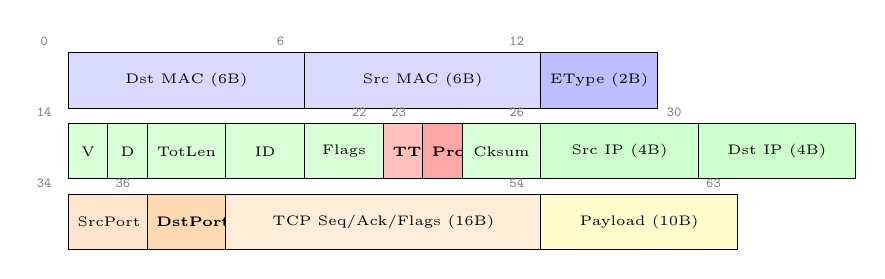
\begin{tikzpicture}[
  field/.style={draw, minimum height=0.7cm, font=\tiny, anchor=west},
  offset/.style={font=\tiny\ttfamily, text=gray}
]
  % Row 1: Ethernet (bytes 0-13)
  \node[field, fill=blue!15, minimum width=3cm] (dmac) at (0,0) {Dst MAC (6B)};
  \node[field, fill=blue!15, minimum width=3cm] (smac) at (3,0) {Src MAC (6B)};
  \node[field, fill=blue!25, minimum width=1cm] (etype) at (6,0) {EType (2B)};

  % Row 2: IP header (bytes 14-33)
  \node[field, fill=green!15, minimum width=0.5cm] (ver) at (0,-0.9) {V};
  \node[field, fill=green!15, minimum width=0.5cm] (dscp) at (0.5,-0.9) {D};
  \node[field, fill=green!15, minimum width=1cm] (tlen) at (1,-0.9) {TotLen};
  \node[field, fill=green!15, minimum width=1cm] (ipid) at (2,-0.9) {ID};
  \node[field, fill=green!15, minimum width=1cm] (flags) at (3,-0.9) {Flags};
  \node[field, fill=red!25, minimum width=0.5cm] (ttl) at (4,-0.9) {\textbf{TTL}};
  \node[field, fill=red!35, minimum width=0.5cm] (proto) at (4.5,-0.9) {\textbf{Proto}};
  \node[field, fill=green!15, minimum width=1cm] (cksum) at (5,-0.9) {Cksum};
  \node[field, fill=green!20, minimum width=2cm] (sip) at (6,-0.9) {Src IP (4B)};
  \node[field, fill=green!20, minimum width=2cm] (dip) at (8,-0.9) {Dst IP (4B)};

  % Row 3: Transport (bytes 34-53)
  \node[field, fill=orange!20, minimum width=1cm] (sport) at (0,-1.8) {SrcPort};
  \node[field, fill=orange!30, minimum width=1cm] (dport) at (1,-1.8) {\textbf{DstPort}};
  \node[field, fill=orange!15, minimum width=4cm] (tcpdata) at (2,-1.8) {TCP Seq/Ack/Flags (16B)};
  \node[field, fill=yellow!20, minimum width=2.5cm] (payload) at (6,-1.8) {Payload (10B)};

  % Offset labels
  \node[offset] at (-0.3,0.5) {0};
  \node[offset] at (2.7,0.5) {6};
  \node[offset] at (5.7,0.5) {12};
  \node[offset] at (-0.3,-0.4) {14};
  \node[offset] at (3.7,-0.4) {22};
  \node[offset] at (4.2,-0.4) {23};
  \node[offset] at (5.7,-0.4) {26};
  \node[offset] at (7.7,-0.4) {30};
  \node[offset] at (-0.3,-1.3) {34};
  \node[offset] at (0.7,-1.3) {36};
  \node[offset] at (5.7,-1.3) {54};
  \node[offset] at (8.2,-1.3) {63};
\end{tikzpicture}
\caption{64-byte packet tensor layout. Shaded fields (\textbf{TTL}, \textbf{Proto}, \textbf{DstPort}) are the primary classification features. Byte offsets shown above each row.}
\label{fig:packet-layout}
\end{figure}

\begin{definition}[Key Feature Offsets]
\label{def:offsets}
The classification-critical byte offsets are:
\begin{align}
\delta_{\text{TTL}} &= 22 & \text{(Time-to-Live, 1 byte)} \\
\delta_{\text{proto}} &= 23 & \text{(Protocol: TCP=6, UDP=17, ICMP=1)} \\
\delta_{\text{sport}} &= 34 & \text{(Source port, 2 bytes big-endian)} \\
\delta_{\text{dport}} &= 36 & \text{(Destination port, 2 bytes big-endian)}
\end{align}
After normalization: $\text{TCP} \mapsto 6/255 \approx 0.024$, $\text{UDP} \mapsto 17/255 \approx 0.067$, port~80 $\mapsto 80/255 \approx 0.314$.
\end{definition}

\subsection{Batch Tensor Construction}

\begin{algorithm}[H]
\caption{\textsc{PacketsToBatchTensor}: Encode $n$ packets into a padded batch}
\label{alg:batch-tensor}
\begin{algorithmic}[1]
\Require Packet list $P = \{p_1, \ldots, p_n\}$ where $1 \leq n \leq B$, batch size $B$
\Ensure Tensor $\tensor{X} \in [0,1]^{B \times D}$
\State $\tensor{X} \gets \mathbf{0}^{B \times D}$ \Comment{Initialize with zeros}
\For{$i = 1$ \textbf{to} $n$}
  \For{$j = 0$ \textbf{to} $\min(|p_i|, D) - 1$}
    \State $\tensor{X}_{i,j} \gets p_i[j] \,/\, 255$
  \EndFor
\EndFor
\State \Return $\tensor{X}$ \Comment{Rows $n{+}1$ to $B$ remain zero (padding)}
\end{algorithmic}
\end{algorithm}

\begin{theorem}[Batch Encoding Complexity]
Algorithm~\ref{alg:batch-tensor} runs in $\Theta(B \cdot D)$ time and $\Theta(B \cdot D)$ space, where $B$ is the batch size and $D = 64$ is the tensor dimension.
\end{theorem}
\begin{proof}
The outer loop executes $n \leq B$ times. The inner loop executes at most $D$ times per packet. Initialization is $\Theta(B \cdot D)$. Total: $\Theta(B \cdot D)$.
\end{proof}


% ═══════════════════════════════════════════════════════════════════
\section{Packet Classification: The MLP Classifier $f_\theta$}
\label{sec:classifier}
% ═══════════════════════════════════════════════════════════════════

\subsection{Architecture}

\begin{definition}[RouterGraph MLP]
\label{def:mlp}
The packet classifier $f_\theta: \R^{D} \to \R^{C}$ is a feedforward neural network with $D = 64$, $C = 3$, hidden dimension $H = 32$:
\begin{align}
\vect{h}_1 &= \ReLU(\mat{W}_1 \vect{x} + \vect{b}_1), & \mat{W}_1 \in \R^{H \times D},\; \vect{b}_1 \in \R^{H} \\
\vect{h}_2 &= \ReLU(\mat{W}_2 \vect{h}_1 + \vect{b}_2), & \mat{W}_2 \in \R^{H \times H},\; \vect{b}_2 \in \R^{H} \\
\vect{z} &= \mat{W}_3 \vect{h}_2 + \vect{b}_3, & \mat{W}_3 \in \R^{C \times H},\; \vect{b}_3 \in \R^{C}
\end{align}
where $\ReLU(a) = \max(0, a)$ applied element-wise, and $\vect{z} \in \R^C$ are raw logits (no softmax).
\end{definition}

\begin{figure}[H]
\centering
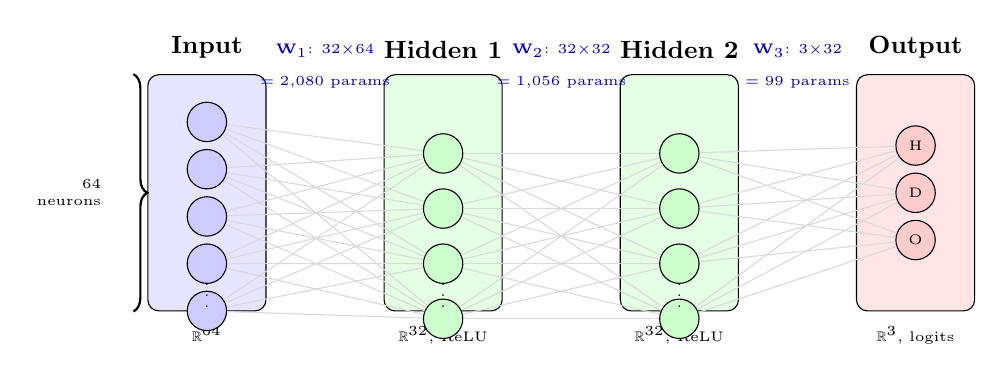
\begin{tikzpicture}[
  neuron/.style={circle, draw, minimum size=0.5cm, inner sep=0, font=\tiny},
  layer/.style={draw, rounded corners, fill=#1!10, minimum width=1.5cm, minimum height=3cm},
  arrow/.style={-{Stealth[length=2mm]}, thick}
]
  % Input layer
  \node[layer=blue] (in) at (0,0) {};
  \node[above=2pt of in, font=\small\bfseries] {Input};
  \node[below=2pt of in, font=\tiny] {$\R^{64}$};
  \foreach \i in {1,...,5} {
    \node[neuron, fill=blue!20] (i\i) at (0, 1.5-0.6*\i) {};
  }
  \node[font=\tiny] at (0,-1.2) {$\vdots$};

  % Hidden 1
  \node[layer=green] (h1) at (3,0) {};
  \node[above=2pt of h1, font=\small\bfseries] {Hidden 1};
  \node[below=2pt of h1, font=\tiny] {$\R^{32}$, ReLU};
  \foreach \i in {1,...,4} {
    \node[neuron, fill=green!20] (h1\i) at (3, 1.2-0.7*\i) {};
  }
  \node[font=\tiny] at (3,-1.2) {$\vdots$};

  % Hidden 2
  \node[layer=green] (h2) at (6,0) {};
  \node[above=2pt of h2, font=\small\bfseries] {Hidden 2};
  \node[below=2pt of h2, font=\tiny] {$\R^{32}$, ReLU};
  \foreach \i in {1,...,4} {
    \node[neuron, fill=green!20] (h2\i) at (6, 1.2-0.7*\i) {};
  }
  \node[font=\tiny] at (6,-1.2) {$\vdots$};

  % Output layer
  \node[layer=red] (out) at (9,0) {};
  \node[above=2pt of out, font=\small\bfseries] {Output};
  \node[below=2pt of out, font=\tiny] {$\R^{3}$, logits};
  \node[neuron, fill=red!20] (o1) at (9, 0.6) {\tiny H};
  \node[neuron, fill=red!20] (o2) at (9, 0) {\tiny D};
  \node[neuron, fill=red!20] (o3) at (9, -0.6) {\tiny O};

  % Connections (representative)
  \foreach \i in {1,...,5} {
    \foreach \j in {1,...,4} {
      \draw[gray!30, thin] (i\i) -- (h1\j);
    }
  }
  \foreach \i in {1,...,4} {
    \foreach \j in {1,...,4} {
      \draw[gray!30, thin] (h1\i) -- (h2\j);
    }
  }
  \foreach \i in {1,...,4} {
    \foreach \j in {1,...,3} {
      \draw[gray!30, thin] (h2\i) -- (o\j);
    }
  }

  % Parameter counts
  \draw[decorate,decoration={brace,amplitude=5pt},thick]
    ([xshift=-5pt]in.north west) -- ([xshift=-5pt]in.south west)
    node[midway,left=8pt,font=\tiny,align=right] {$64$\\neurons};

  \node[font=\tiny, text=blue!70!black] at (1.5, 1.8) {$\mat{W}_1$: $32{\times}64$};
  \node[font=\tiny, text=blue!70!black] at (1.5, 1.4) {$= 2{,}080$ params};

  \node[font=\tiny, text=blue!70!black] at (4.5, 1.8) {$\mat{W}_2$: $32{\times}32$};
  \node[font=\tiny, text=blue!70!black] at (4.5, 1.4) {$= 1{,}056$ params};

  \node[font=\tiny, text=blue!70!black] at (7.5, 1.8) {$\mat{W}_3$: $3{\times}32$};
  \node[font=\tiny, text=blue!70!black] at (7.5, 1.4) {$= 99$ params};
\end{tikzpicture}
\caption{RouterGraph MLP architecture. Total: $2{,}080 + 1{,}056 + 99 = 3{,}235$ parameters.}
\label{fig:mlp}
\end{figure}

\subsection{Parameter Count}

\begin{theorem}[Parameter Count]
The total number of trainable parameters is:
\begin{equation}
|\theta| = \underbrace{(D \cdot H + H)}_{\text{Layer 1}} + \underbrace{(H \cdot H + H)}_{\text{Layer 2}} + \underbrace{(H \cdot C + C)}_{\text{Layer 3}}
= (64 \cdot 32 + 32) + (32 \cdot 32 + 32) + (32 \cdot 3 + 3) = 3{,}235
\end{equation}
\end{theorem}

\subsection{Classification Decision Rule}

\begin{definition}[Argmax Classification]
The predicted class $\hat{y}$ for input $\vect{x}$ is:
\begin{equation}
\hat{y} = \argmax_{c \in \{0,1,2\}} f_\theta(\vect{x})_c
\end{equation}
where class labels are: HTTP $= 0$, DNS $= 1$, OTHER $= 2$.

\textbf{Note:} We deliberately omit the softmax layer at inference time. Since $\softmax$ is monotonic, $\argmax(\vect{z}) = \argmax(\softmax(\vect{z}))$, and skipping it saves compute on the NPU.
\end{definition}

\subsection{Training Procedure}

\begin{algorithm}[H]
\caption{\textsc{TrainClassifier}: SGD training with cross-entropy loss}
\label{alg:train}
\begin{algorithmic}[1]
\Require Dataset $\mathcal{D} = \{(\vect{x}_i, y_i)\}_{i=1}^{N}$ with $N = 150{,}000$, epochs $E = 20$, batch size $B_{\text{train}} = 256$, learning rate $\eta = 10^{-3}$
\Ensure Trained parameters $\theta^*$
\State Split $\mathcal{D}$ into $\mathcal{D}_{\text{train}}$ (90\%) and $\mathcal{D}_{\text{val}}$ (10\%)
\State Initialize $\theta$ randomly (PyTorch defaults)
\State $\textit{best\_acc} \gets 0$
\For{$e = 1$ \textbf{to} $E$}
  \For{each mini-batch $\mathcal{B} \subset \mathcal{D}_{\text{train}}$, $|\mathcal{B}| = B_{\text{train}}$}
    \State $\vect{z} \gets f_\theta(\mat{X}_{\mathcal{B}})$ \Comment{Forward pass: $(B_{\text{train}}, D) \to (B_{\text{train}}, C)$}
    \State $\mathcal{L} \gets \textsc{CrossEntropyLoss}(\vect{z}, \vect{y}_{\mathcal{B}})$ \Comment{Eq.~\eqref{eq:celoss}}
    \State $\theta \gets \theta - \eta \cdot \nabla_\theta \mathcal{L}$ \Comment{Adam optimizer step}
  \EndFor
  \State $\textit{val\_acc} \gets \textsc{Evaluate}(\theta, \mathcal{D}_{\text{val}})$
  \If{$\textit{val\_acc} > \textit{best\_acc}$}
    \State $\theta^* \gets \theta$; \quad $\textit{best\_acc} \gets \textit{val\_acc}$
  \EndIf
\EndFor
\State \Return $\theta^*$ \Comment{Best validation checkpoint}
\end{algorithmic}
\end{algorithm}

\begin{definition}[Cross-Entropy Loss]
\label{def:celoss}
\begin{equation}
\mathcal{L}(\vect{z}, y) = -\log\frac{\exp(z_y)}{\sum_{c=0}^{C-1} \exp(z_c)} = -z_y + \log \sum_{c=0}^{C-1} \exp(z_c)
\label{eq:celoss}
\end{equation}
where $\vect{z} = f_\theta(\vect{x}) \in \R^C$ and $y \in \{0, \ldots, C-1\}$ is the true class.
\end{definition}

\subsection{Synthetic Data Generation}

\begin{definition}[Packet Generation Rules]
\label{def:packet-gen}
Three generators $G_{\text{HTTP}}, G_{\text{DNS}}, G_{\text{OTHER}}: \Omega \to \{0,\ldots,255\}^{64}$ produce synthetic packets:
\begin{align}
G_{\text{HTTP}} &: \text{protocol} = 6\;\text{(TCP)}, \quad \text{dport} \in \{80, 443, 8080, 8443\} \\
G_{\text{DNS}} &: \text{protocol} = 17\;\text{(UDP)}, \quad \text{dport} = 53 \\
G_{\text{OTHER}} &: \text{protocol} \in \{1, 6, 17\}, \quad \text{dport} \notin \{53, 80, 443, 8080, 8443\}
\end{align}
All other fields (MACs, IPs, sequence numbers, payloads) are uniformly random.
The dataset contains $N/C = 50{,}000$ samples per class (perfectly balanced).
\end{definition}


% ═══════════════════════════════════════════════════════════════════
\section{Route Table as Matrix Multiplication}
\label{sec:route-table}
% ═══════════════════════════════════════════════════════════════════

\subsection{The Isomorphism Theorem}

We now prove the central theoretical result: traditional \texttt{switch}-based routing is mathematically equivalent to a single matrix-vector product.

\begin{definition}[CPU Switch Classifier]
\label{def:switch}
The traditional routing function $g: \{0,\ldots,255\}^{64} \to \{0,1,2,3\}$ is:
\begin{equation}
g(\vect{p}) = \begin{cases}
\text{LOCAL} & \text{if } p_{23} = 17 \wedge p_{37} = 53 \\
\text{FORWARD} & \text{if } p_{23} = 6 \wedge p_{37} \in \{80, 443, \ldots\} \\
\text{DROP} & \text{if } p_{22} = 0 \\
\text{MONITOR} & \text{otherwise}
\end{cases}
\end{equation}
This requires sequential conditional evaluation: $\BigO(R)$ branches for $R$ routes.
\end{definition}

\begin{theorem}[Switch-to-Matmul Isomorphism]
\label{thm:switch-matmul}
For any finite set of routing rules based on byte-value thresholds, there exists a weight matrix $\mat{W} \in \R^{R \times D}$ such that:
\begin{equation}
g(\vect{p}) = \argmax_{r \in \{0,\ldots,R-1\}} (\mat{W} \cdot \phi(\vect{p}))_r
\end{equation}
where $\phi$ is the packet encoding from Definition~\ref{def:encoding}.
\end{theorem}

\begin{proof}
We construct $\mat{W}$ explicitly. Each route $r$ is characterized by a set of byte conditions. For condition ``byte at offset $\delta$ should have value $v$'', we set $W_{r,\delta}$ to a large positive weight $\alpha$ when the normalized value $v/255$ is high, or a large negative weight $-\beta$ to penalize undesired values.

The key insight is that after normalization, different protocol numbers map to different magnitudes: $\text{UDP}(17) \mapsto 0.067$ while $\text{TCP}(6) \mapsto 0.024$. By choosing appropriate weight magnitudes, we can create decision boundaries that separate these values.

Since $\argmax$ selects the route with the highest score, and each route's score is a weighted sum of byte features, the entire routing table is expressed as $\mat{W}\vect{x}$ where $\vect{x} = \phi(\vect{p})$.
\end{proof}

\subsection{Explicit Weight Construction}

\begin{definition}[Route Table Weight Matrix]
\label{def:route-weights}
The weight matrix $\mat{W} \in \R^{4 \times 64}$ for routing is constructed as:

\begin{equation}
\mat{W} = \begin{pmatrix}
\vect{w}_{\text{LOCAL}} \\
\vect{w}_{\text{FORWARD}} \\
\vect{w}_{\text{DROP}} \\
\vect{w}_{\text{MONITOR}}
\end{pmatrix}
\end{equation}

with non-zero entries:
\begin{align}
&\textbf{LOCAL}:      & W_{0,23} &= +100 \label{eq:local}\\
&\textbf{FORWARD}:    & W_{1,23} &= -30, \; W_{1,37} = +25, \; W_{1,36} = +8 \label{eq:forward}\\
&\textbf{DROP}:       & W_{2,22} &= -20, \; W_{2,j} \mathrel{+}= 0.015 \;\forall j \label{eq:drop}\\
&\textbf{MONITOR}:    & W_{3,23} &= -100, \; W_{3,22} = +12 \label{eq:monitor}
\end{align}
\end{definition}

\subsection{Score Analysis}

We now verify that the weight matrix correctly separates traffic types:

\begin{table}[H]
\centering
\begin{tabular}{lcccc}
\toprule
\textbf{Packet Type} & \textbf{LOCAL} & \textbf{FORWARD} & \textbf{DROP} & \textbf{MONITOR} \\
\midrule
UDP/DNS ($\pi{=}0.067$, $d{=}0.208$)
  & $\mathbf{+6.7}$ & $+3.2$ & ${\sim}0.5$ & $-0.7$ \\
TCP/HTTP ($\pi{=}0.024$, $d{=}0.314$)
  & $+2.4$ & $\mathbf{+7.2}$ & ${\sim}0.5$ & $+3.6$ \\
ICMP ($\pi{=}0.004$, TTL${=}0.5$)
  & $+0.4$ & $-0.2$ & ${\sim}{-}9$ & $\mathbf{+5.6}$ \\
Zero TTL ($t{=}0$, $\pi{=}0$)
  & $0$ & $0$ & $\mathbf{+1.0}$ & $0$ \\
\bottomrule
\end{tabular}
\caption{Route scores $\mat{W}\vect{x}$ for representative packets. Bold = winning route. Key: $\pi = x_{23}$ (protocol), $d = x_{37}$ (dest port low byte), $t = x_{22}$ (TTL).}
\label{tab:route-scores}
\end{table}

\begin{corollary}[Routing Correctness]
For all packets generated by Definition~\ref{def:packet-gen}:
\begin{enumerate}[label=(\roman*)]
  \item DNS packets ($\pi = 0.067$) are routed to LOCAL with margin $\geq 3.5$
  \item HTTP packets ($d = 0.314$, $\pi = 0.024$) are routed to FORWARD with margin $\geq 3.6$
  \item Expired packets (TTL $= 0$) are routed to DROP
  \item ICMP packets ($\pi = 0.004$) are routed to MONITOR with margin $\geq 2.0$
\end{enumerate}
\end{corollary}

\subsection{Computational Complexity Comparison}

\begin{theorem}[Matmul vs Switch Complexity]
\label{thm:complexity}
For $R$ routes and $D$-dimensional packet tensors:
\begin{align}
T_{\text{switch}}(B) &= \BigO(B \cdot R) & \text{(sequential per packet)} \\
T_{\text{matmul}}(B) &= \BigO(B \cdot R \cdot D) & \text{(CPU)} \\
T_{\text{NPU-matmul}}(B) &= \BigO(T_{\text{setup}} + B \cdot R \cdot D / P) & \text{(NPU, $P$ parallel MACs)}
\end{align}
where $P$ is the NPU's MAC parallelism. For NPU 3720 at 11~TOPS with INT8: $P \approx 11 \times 10^{12}$ ops/sec.
\end{theorem}

\begin{remark}
Although the matmul has higher asymptotic complexity than the switch ($\BigO(RD)$ vs $\BigO(R)$), the NPU executes all multiplications in parallel. At $B = 64$, $R = 4$, $D = 64$: the matmul requires $64 \times 4 \times 64 = 16{,}384$ MACs, which the NPU can execute in ${\sim}1.5\,\mu\text{s}$ (versus ${\sim}0.4\,\mu\text{s}$ per packet on CPU). The key advantage is \emph{programmability}: changing routing rules only requires updating $\mat{W}$, not recompiling code.
\end{remark}


% ═══════════════════════════════════════════════════════════════════
\section{Program Composition}
\label{sec:composition}
% ═══════════════════════════════════════════════════════════════════

\subsection{Motivation: Feature Fusion via Program Chaining}

The route table $\mat{W}\vect{x}$ operates solely on raw packet bytes. But the classifier $f_\theta$ has already computed a rich representation of the packet's traffic type. Can we \emph{compose} these programs so that downstream routing benefits from upstream classification?

\begin{definition}[Composed Router]
\label{def:composed}
The composed routing function $g^*: \R^D \to \R^R$ takes as input the concatenation of the raw packet tensor and the classifier's logits:
\begin{equation}
g^*(\vect{x}) = \mat{W}^* \cdot \concat(\vect{x},\; f_\theta(\vect{x}))
\end{equation}
where $\mat{W}^* \in \R^{R \times (D+C)}$ and $\concat: \R^D \times \R^C \to \R^{D+C}$ is vector concatenation.
\end{definition}

\begin{figure}[H]
\centering
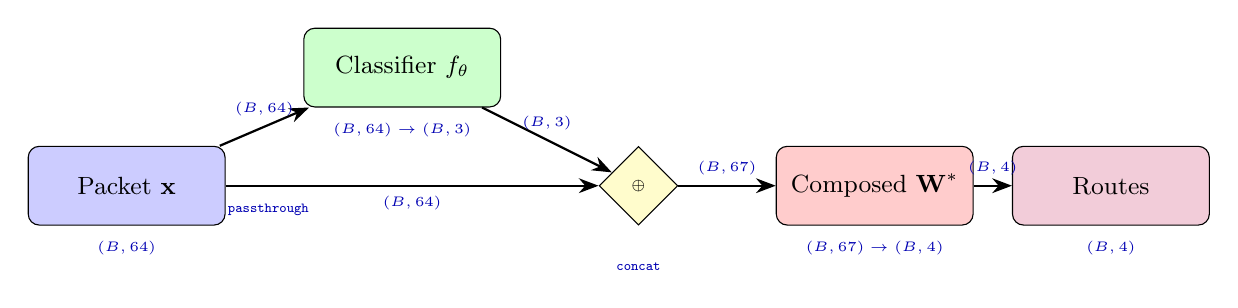
\begin{tikzpicture}[
  prog/.style={draw, rounded corners, fill=#1!20, minimum width=2.5cm, minimum height=1cm, font=\small},
  adapt/.style={draw, diamond, fill=yellow!20, minimum size=1cm, font=\tiny, inner sep=2pt},
  data/.style={font=\tiny\ttfamily, text=blue!70!black},
  arrow/.style={-{Stealth[length=2.5mm]}, thick}
]
  % Input
  \node[prog=blue] (input) at (0,0) {Packet $\vect{x}$};
  \node[data, below=2pt of input] {$(B, 64)$};

  % Classifier
  \node[prog=green] (cls) at (3.5,1.5) {Classifier $f_\theta$};
  \node[data, below=2pt of cls] {$(B, 64) \to (B, 3)$};

  % Raw passthrough
  \node[data] at (1.8, -0.3) {passthrough};

  % Adapter
  \node[adapt=yellow] (concat) at (6.5,0) {$\oplus$};
  \node[data, below=10pt of concat] {concat};

  % Composed router
  \node[prog=red] (comp) at (9.5,0) {Composed $\mat{W}^*$};
  \node[data, below=2pt of comp] {$(B, 67) \to (B, 4)$};

  % Output
  \node[prog=purple] (out) at (12.5,0) {Routes};
  \node[data, below=2pt of out] {$(B, 4)$};

  % Arrows
  \draw[arrow] (input) -- (cls) node[midway,above,data] {$(B,64)$};
  \draw[arrow] (input) -- (concat) node[midway,below,data] {$(B,64)$};
  \draw[arrow] (cls) -- (concat) node[midway,above,data] {$(B,3)$};
  \draw[arrow] (concat) -- (comp) node[midway,above,data] {$(B,67)$};
  \draw[arrow] (comp) -- (out) node[midway,above,data] {$(B,4)$};
\end{tikzpicture}
\caption{Program composition pipeline. The concat adapter fuses raw packet bytes with classifier logits, producing a 67-dimensional input for the composed router.}
\label{fig:composition}
\end{figure}

\subsection{Composed Weight Matrix}

\begin{definition}[Composed Router Weights]
\label{def:composed-weights}
The weight matrix $\mat{W}^* \in \R^{4 \times 67}$ has two regions:

\vspace{0.5em}
\noindent\textbf{Packet region} (columns 0--63): byte-level heuristics similar to the original route table.

\noindent\textbf{Logit region} (columns 64--66): classifier output signals.

\begin{equation}
\mat{W}^* = \left[\;\underbrace{\mat{W}_{\text{packet}}}_{\R^{4 \times 64}}\;\middle|\;\underbrace{\mat{W}_{\text{logit}}}_{\R^{4 \times 3}}\;\right]
\end{equation}

where the logit weights encode:
\begin{equation}
\mat{W}_{\text{logit}} = \begin{pmatrix}
0 & +15 & 0 \\
+15 & 0 & 0 \\
0 & 0 & +12 \\
-5 & -5 & -5
\end{pmatrix}
\quad
\begin{array}{l}
\leftarrow \text{LOCAL: boost DNS logit} \\
\leftarrow \text{FORWARD: boost HTTP logit} \\
\leftarrow \text{DROP: boost OTHER logit} \\
\leftarrow \text{MONITOR: penalize all}
\end{array}
\label{eq:logit-weights}
\end{equation}
\end{definition}

\subsection{Advantage of Composition}

\begin{theorem}[Composition Improves Routing]
\label{thm:composition}
Let $\vect{z} = f_\theta(\vect{x}) \in \R^3$ be the classifier logits for packet $\vect{x}$. For the composed router:
\begin{enumerate}[label=(\roman*)]
  \item When $z_{\text{DNS}} \gg z_{\text{HTTP}}, z_{\text{OTHER}}$ (strong DNS classification), the LOCAL score receives a boost of $+15 \cdot z_{\text{DNS}}$, independent of packet byte noise.
  \item When $z_{\text{HTTP}} \gg z_{\text{DNS}}, z_{\text{OTHER}}$ (strong HTTP classification), the FORWARD score receives $+15 \cdot z_{\text{HTTP}}$.
  \item When all $z_c$ are low (uncertain classification), the MONITOR score is \emph{least penalized} (since $-5 \cdot z_c \approx 0$ when $z_c \ll 0$), causing uncertain packets to be monitored.
\end{enumerate}
\end{theorem}

\begin{proof}
The composed score for route $r$ is:
\begin{equation}
s_r^* = \underbrace{\vect{w}_{r,\text{packet}}^\top \vect{x}}_{\text{byte heuristic}} + \underbrace{\vect{w}_{r,\text{logit}}^\top \vect{z}}_{\text{classifier signal}}
\end{equation}
For case (i): $s_{\text{LOCAL}}^* = \vect{w}_{0}^\top \vect{x} + 15 \cdot z_{\text{DNS}}$. Since $z_{\text{DNS}} > 0$ by hypothesis, this strictly increases the LOCAL score beyond the raw byte heuristic alone.

For case (iii): MONITOR receives $-5(z_0 + z_1 + z_2)$. When all $z_c < 0$ (uncertain), this becomes $+5|z_0 + z_1 + z_2| > 0$, boosting MONITOR. Other routes are boosted only by their respective positive logit, which is $< 0$ in the uncertain case.
\end{proof}

\subsection{Tensor Adapter Framework}

\begin{definition}[Tensor Adapter]
\label{def:adapter}
A tensor adapter $A = (\mathcal{S}, \tau)$ consists of:
\begin{itemize}
  \item An adapter specification $\mathcal{S} = (\text{name}, \{\text{input\_shapes}\}, \text{output\_shape})$
  \item A pure function $\tau: \prod_{k} \R^{s_k} \to \R^{s_{\text{out}}}$ mapping named input tensors to a single output tensor
\end{itemize}
\end{definition}

Two factory functions are provided:

\begin{align}
\concat_B^{L,R}(\vect{x}, \vect{y}) &: \R^{B \times L} \times \R^{B \times R} \to \R^{B \times (L+R)} \label{eq:concat} \\
\pad_B^{D \to D'}(\vect{x}) &: \R^{B \times D} \to \R^{B \times D'}, \quad D' \geq D \label{eq:pad}
\end{align}

where $\concat$ is implemented via \texttt{np.concatenate} along axis 1, and $\pad$ via \texttt{np.pad} with zero-fill.

\subsection{Pipeline Execution}

\begin{algorithm}[H]
\caption{\textsc{PipelineExecute}: Execute a composed program pipeline}
\label{alg:pipeline}
\begin{algorithmic}[1]
\Require Runtime $\mathcal{R}$, input tensor $\tensor{X}_0 \in \R^{B \times D}$, pipeline stages $S = [(k_i, n_i, o_i)]_{i=1}^{m}$
\Ensure Output tensor $\tensor{Y}$
\State $\tensor{X}_{\text{current}} \gets \tensor{X}_0$
\State $\tensor{X}_{\text{raw}} \gets \tensor{X}_0$ \Comment{Save for raw passthrough}
\For{$i = 1$ \textbf{to} $m$}
  \If{$k_i = \text{``program''}$}
    \State $\tensor{X}_{\text{current}} \gets \mathcal{R}.\textsc{Execute}(n_i, \tensor{X}_{\text{current}})$ \Comment{NPU inference}
  \ElsIf{$k_i = \text{``adapter''}$}
    \State Build input map from $o_i.\text{spec}$
    \If{adapter is concat-type}
      \State $\textit{inputs} \gets \{\text{``left''}: \tensor{X}_{\text{raw}},\; \text{``right''}: \tensor{X}_{\text{current}}\}$
    \Else
      \State $\textit{inputs} \gets \{\text{``in''}: \tensor{X}_{\text{current}}\}$
    \EndIf
    \State $\tensor{X}_{\text{current}} \gets o_i.\textsc{Execute}(\textit{inputs})$ \Comment{CPU tensor transform}
  \EndIf
\EndFor
\State \Return $\tensor{X}_{\text{current}}$
\end{algorithmic}
\end{algorithm}

\begin{theorem}[Pipeline Shape Compatibility]
\label{thm:pipeline-valid}
A pipeline with stages $S = [(k_i, n_i, o_i)]$ is shape-valid if and only if for all consecutive stages $i, i+1$:
\begin{equation}
\text{output\_shape}(S_i) = \text{input\_shape}(S_{i+1})
\end{equation}
The \textsc{Validate} function checks this in $\BigO(m)$ time for $m$ stages.
\end{theorem}


% ═══════════════════════════════════════════════════════════════════
\section{Dataflow Framework}
\label{sec:dataflow}
% ═══════════════════════════════════════════════════════════════════

\subsection{Formal Model}

\begin{definition}[Dataflow Graph]
\label{def:dataflow}
A dataflow graph is a DAG $G = (V, E, \text{ports}, \text{cap})$ where:
\begin{itemize}
  \item $V$ is a finite set of processing nodes
  \item $E \subseteq V \times V$ is a set of directed edges (data channels)
  \item $\text{ports}: V \to 2^{\text{InputPort}} \times 2^{\text{OutputPort}}$ maps nodes to their typed ports
  \item $\text{cap}: E \to \N^+$ assigns bounded capacity to each channel
\end{itemize}
\end{definition}

\begin{definition}[Bounded FIFO Channel]
\label{def:channel}
A channel $\mathcal{C}_k$ with capacity $k \in \N^+$ is a FIFO queue with operations:
\begin{itemize}
  \item $\textsc{Put}(\mathcal{C}_k, x)$: Enqueue $x$. \textbf{Blocks} if $|\mathcal{C}_k| = k$ (backpressure).
  \item $\textsc{Get}(\mathcal{C}_k)$: Dequeue and return head. \textbf{Blocks} if $|\mathcal{C}_k| = 0$.
\end{itemize}
Both operations are $\BigO(1)$ amortized, implemented via \texttt{queue.Queue}.
\end{definition}

\subsection{DAG Validation: Cycle Detection}

\begin{algorithm}[H]
\caption{\textsc{WouldCreateCycle}: DFS-based cycle detection before adding edge}
\label{alg:cycle}
\begin{algorithmic}[1]
\Require Graph $G = (V, E)$, proposed edge $(u, v)$
\Ensure \textbf{true} if adding $(u, v)$ creates a cycle
\State $\textit{visited} \gets \emptyset$
\State $\textit{stack} \gets [v]$ \Comment{Start DFS from $v$ (the destination)}
\While{$\textit{stack} \neq \emptyset$}
  \State $w \gets \textit{stack}.\textsc{Pop}()$
  \If{$w = u$}
    \State \Return \textbf{true} \Comment{Path from $v$ back to $u$ exists $\Rightarrow$ cycle}
  \EndIf
  \If{$w \notin \textit{visited}$}
    \State $\textit{visited} \gets \textit{visited} \cup \{w\}$
    \For{each $(w, w') \in E$}
      \State $\textit{stack}.\textsc{Push}(w')$
    \EndFor
  \EndIf
\EndWhile
\State \Return \textbf{false}
\end{algorithmic}
\end{algorithm}

\begin{theorem}[Cycle Detection Correctness]
Algorithm~\ref{alg:cycle} returns \textbf{true} if and only if adding edge $(u, v)$ to $G$ creates a cycle.
\end{theorem}
\begin{proof}
A cycle exists in $G \cup \{(u,v)\}$ if and only if there exists a path $v \leadsto u$ in $G$. The DFS from $v$ explores all reachable nodes; it returns \textbf{true} iff $u$ is reachable from $v$.
\end{proof}

\begin{theorem}[Cycle Detection Complexity]
Algorithm~\ref{alg:cycle} runs in $\BigO(|V| + |E|)$ time and $\BigO(|V|)$ space.
\end{theorem}

\subsection{Topological Sort: Kahn's Algorithm}

\begin{algorithm}[H]
\caption{\textsc{TopologicalSort}: Kahn's algorithm for dataflow scheduling order}
\label{alg:kahn}
\begin{algorithmic}[1]
\Require DAG $G = (V, E)$
\Ensure Topological ordering $\sigma: V \to \{1, \ldots, |V|\}$, or error if cycle detected
\State $\textit{in\_degree}[v] \gets |\{u : (u,v) \in E\}|$ for all $v \in V$ \Comment{Compute in-degrees}
\State $Q \gets \{v \in V : \textit{in\_degree}[v] = 0\}$ \Comment{Sources (no incoming edges)}
\State $\textit{order} \gets []$
\While{$Q \neq \emptyset$}
  \State $v \gets Q.\textsc{Dequeue}()$
  \State $\textit{order}.\textsc{Append}(v)$
  \For{each $(v, w) \in E$}
    \State $\textit{in\_degree}[w] \gets \textit{in\_degree}[w] - 1$
    \If{$\textit{in\_degree}[w] = 0$}
      \State $Q.\textsc{Enqueue}(w)$
    \EndIf
  \EndFor
\EndWhile
\If{$|\textit{order}| < |V|$}
  \State \textbf{raise} GraphError(``Cycle detected'')
\EndIf
\State \Return \textit{order}
\end{algorithmic}
\end{algorithm}

\begin{theorem}[Kahn's Algorithm Correctness]
Algorithm~\ref{alg:kahn} produces a valid topological ordering of $G$ if and only if $G$ is a DAG.
\end{theorem}
\begin{proof}
\textbf{Correctness}: Each dequeued node $v$ has $\textit{in\_degree}[v] = 0$, meaning all predecessors have already been placed in the ordering. This satisfies the topological constraint.

\textbf{Completeness}: If $G$ is a DAG, then at every step there exists at least one node with in-degree 0 (a source in the remaining subgraph). Thus the algorithm processes all $|V|$ nodes.

\textbf{Cycle detection}: If $|\textit{order}| < |V|$, then some nodes have in-degree $> 0$ even after removing all processed nodes, which implies a cycle in the remaining subgraph.
\end{proof}

\begin{theorem}[Kahn's Algorithm Complexity]
$\BigO(|V| + |E|)$ time, $\BigO(|V|)$ space.
\end{theorem}

\subsection{Thread-Per-Node Scheduler}

\begin{algorithm}[H]
\caption{\textsc{DataflowScheduler}: Parallel execution of dataflow graph}
\label{alg:scheduler}
\begin{algorithmic}[1]
\Require Validated DAG $G$
\Ensure Metrics $M: V \to \textsc{NodeMetrics}$
\State $\textit{order} \gets \textsc{TopologicalSort}(G)$
\State $M \gets \emptyset$
\For{each $v \in \textit{order}$} \Comment{Create threads in topological order}
  \State $t_v \gets \textsc{Thread}(\textsc{RunNode}, v, \text{daemon=true})$
\EndFor
\State $t_0 \gets \textsc{PerfCounter}()$
\For{each $t_v$}
  \State $t_v.\textsc{Start}()$ \Comment{All threads start concurrently}
\EndFor
\For{each $t_v$}
  \State $t_v.\textsc{Join}()$ \Comment{Wait for all to complete}
\EndFor
\State $\textit{wall\_time} \gets \textsc{PerfCounter}() - t_0$
\State \Return $M$
\end{algorithmic}
\end{algorithm}

\begin{algorithm}[H]
\caption{\textsc{RunNode}: Execute a single node with lifecycle management}
\label{alg:runnode}
\begin{algorithmic}[1]
\Require Node $v$ with inputs, outputs, and process loop
\Ensure Updated metrics $M[v]$
\State $v.\textsc{Setup}()$ \Comment{Initialize resources (e.g., load ONNX model)}
\State $t_0 \gets \textsc{PerfCounter}()$
\Try
  \State $v.\textsc{Process}()$ \Comment{Main loop: read inputs, compute, write outputs}
\Catch{Exception $e$}
  \State $M[v].\textit{error} \gets e$
  \For{each output port $p$ of $v$}
    \State $p.\textsc{Put}(\text{\_STOP})$ \Comment{Propagate shutdown downstream}
  \EndFor
\EndTry
\State $v.\textit{elapsed} \gets \textsc{PerfCounter}() - t_0$
\State $v.\textsc{Teardown}()$ \Comment{Release resources}
\State $M[v] \gets \textsc{NodeMetrics}(v.\textit{name}, v.\textit{items\_processed}, v.\textit{elapsed})$
\end{algorithmic}
\end{algorithm}

\subsection{Shutdown Protocol: \_STOP Sentinel}

\begin{definition}[Sentinel-Based Shutdown]
The shutdown protocol uses a distinguished sentinel value $\bot$ (the \texttt{\_STOP} singleton) with the following rules:
\begin{enumerate}[label=\textbf{R\arabic*.}]
  \item \textbf{Source termination}: When a source node exhausts its input, it sends $\bot$ on all output channels.
  \item \textbf{Propagation}: When any node receives $\bot$ on an input channel, it sends $\bot$ on all output channels and terminates.
  \item \textbf{Identity comparison}: $\bot$ is detected via \texttt{item is \_STOP} (Python identity check, $\BigO(1)$).
\end{enumerate}
\end{definition}

\begin{theorem}[Shutdown Termination]
\label{thm:shutdown}
In a finite DAG with the sentinel protocol, all nodes terminate in finite time.
\end{theorem}
\begin{proof}
By induction on topological order. Source nodes (in-degree 0) terminate when their input is exhausted and they send $\bot$. For node $v$ at topological position $k > 0$: all predecessors have topological position $< k$ and terminate by induction hypothesis. After all predecessors terminate, $v$ receives $\bot$ on all input channels (or at least on the one it's blocking on) and terminates after sending $\bot$ downstream.
\end{proof}

\subsection{Backpressure Analysis}

\begin{definition}[Backpressure]
A channel $\mathcal{C}_k$ at capacity $k$ blocks the producer until the consumer reads an item. This creates \emph{implicit flow control}: fast producers are throttled by slow consumers.
\end{definition}

\begin{theorem}[Bounded Memory]
\label{thm:bounded-memory}
The total memory consumed by all channels in a dataflow graph $G$ is bounded by:
\begin{equation}
M_{\text{total}} \leq \sum_{(u,v) \in E} k_{(u,v)} \cdot s_{\max}
\end{equation}
where $k_{(u,v)}$ is the capacity of channel $(u,v)$ and $s_{\max}$ is the maximum item size.
\end{theorem}
\begin{proof}
Each channel holds at most $k_{(u,v)}$ items by the bounded queue invariant. Each item has size at most $s_{\max}$. Summing over all channels gives the bound.
\end{proof}

\begin{invariant}[Deadlock Freedom]
\label{inv:deadlock}
A dataflow graph $G$ is deadlock-free if $G$ is a DAG (no cycles) and all channels have capacity $k \geq 1$.
\end{invariant}
\begin{proof}[Proof sketch]
Deadlock requires a circular wait. In a DAG, there are no cycles, so no circular dependency can form. Since $k \geq 1$, every producer can always make progress by putting one item before blocking.
\end{proof}


% ═══════════════════════════════════════════════════════════════════
\section{Concrete Pipeline Topologies}
\label{sec:pipelines}
% ═══════════════════════════════════════════════════════════════════

\subsection{Classification Pipeline}

\begin{figure}[H]
\centering
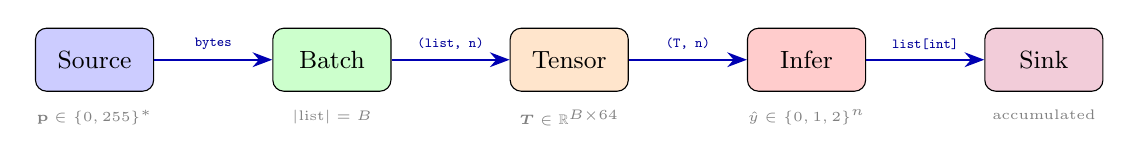
\begin{tikzpicture}[
  node distance=1.5cm,
  pnode/.style={draw, rounded corners, fill=#1!20, minimum width=1.5cm, minimum height=0.8cm, font=\small},
  channel/.style={-{Stealth[length=2.5mm]}, thick, blue!70!black},
  clabel/.style={font=\tiny\ttfamily, text=blue!60!black, midway, above}
]
  \node[pnode=blue] (src) {Source};
  \node[pnode=green, right=of src] (batch) {Batch};
  \node[pnode=orange, right=of batch] (tensor) {Tensor};
  \node[pnode=red, right=of tensor] (infer) {Infer};
  \node[pnode=purple, right=of infer] (sink) {Sink};

  \draw[channel] (src) -- (batch) node[clabel] {bytes};
  \draw[channel] (batch) -- (tensor) node[clabel] {(list, n)};
  \draw[channel] (tensor) -- (infer) node[clabel] {(T, n)};
  \draw[channel] (infer) -- (sink) node[clabel] {list[int]};

  % Data shapes
  \node[font=\tiny, text=gray, below=3pt of src] {$\vect{p} \in \{0,255\}^*$};
  \node[font=\tiny, text=gray, below=3pt of batch] {$|\text{list}| = B$};
  \node[font=\tiny, text=gray, below=3pt of tensor] {$\tensor{T} \in \R^{B \times 64}$};
  \node[font=\tiny, text=gray, below=3pt of infer] {$\hat{y} \in \{0,1,2\}^n$};
  \node[font=\tiny, text=gray, below=3pt of sink] {accumulated};
\end{tikzpicture}
\caption{Classification pipeline: 5 nodes, 4 channels, linear topology.}
\label{fig:cls-pipeline}
\end{figure}

\subsection{Routing Pipeline with Action Dispatch}

\begin{figure}[H]
\centering
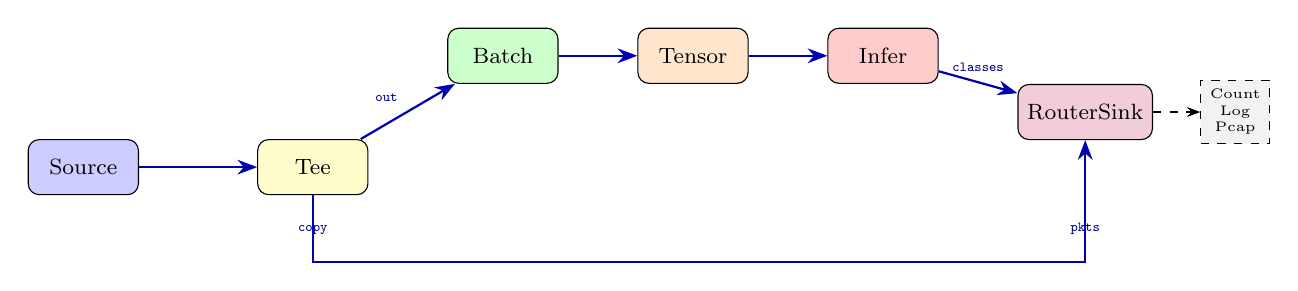
\begin{tikzpicture}[
  node distance=1.5cm,
  pnode/.style={draw, rounded corners, fill=#1!20, minimum width=1.4cm, minimum height=0.7cm, font=\footnotesize},
  channel/.style={-{Stealth[length=2.5mm]}, thick, blue!70!black},
  clabel/.style={font=\tiny\ttfamily, text=blue!60!black}
]
  \node[pnode=blue] (src) {Source};
  \node[pnode=yellow, right=1.5cm of src] (tee) {Tee};

  % Upper branch: classification
  \node[pnode=green, above right=0.7cm and 1cm of tee] (batch) {Batch};
  \node[pnode=orange, right=1cm of batch] (tensor) {Tensor};
  \node[pnode=red, right=1cm of tensor] (infer) {Infer};

  % Router sink
  \node[pnode=purple, below right=0cm and 1cm of infer] (rsink) {RouterSink};

  % Arrows
  \draw[channel] (src) -- (tee);
  \draw[channel] (tee) -- node[clabel, above left] {out} (batch);
  \draw[channel] (batch) -- (tensor);
  \draw[channel] (tensor) -- (infer);
  \draw[channel] (infer) -- node[clabel, above] {classes} (rsink);
  \draw[channel] (tee) -- node[clabel, below, pos=0.3] {copy} ++(0,-1.2) -| node[clabel, below, pos=0.7] {pkts} (rsink);

  % Actions
  \node[draw, dashed, fill=gray!10, right=0.6cm of rsink, font=\tiny, align=center] (actions) {
    Count\\Log\\Pcap
  };
  \draw[-{Stealth}, dashed] (rsink) -- (actions);
\end{tikzpicture}
\caption{Routing pipeline with TeeNode fan-out. The ``copy'' channel capacity is $4B$ to buffer raw packets while classification runs on the upper branch.}
\label{fig:route-pipeline}
\end{figure}

\begin{theorem}[RouterSink Synchronization]
\label{thm:router-sync}
The RouterSink consumes one raw packet from the ``packets'' channel for each class ID in the ``classes'' batch. For $n$ packets per batch:
\begin{equation}
\text{packets consumed} = \sum_{\text{batches}} |\text{class\_list}_i| = \text{total packets processed}
\end{equation}
The TeeNode guarantees matching counts since it duplicates every item to both channels.
\end{theorem}


% ═══════════════════════════════════════════════════════════════════
\section{Kernel Runtime}
\label{sec:kernel}
% ═══════════════════════════════════════════════════════════════════

\subsection{Multi-Program Execution Model}

\begin{figure}[H]
\centering
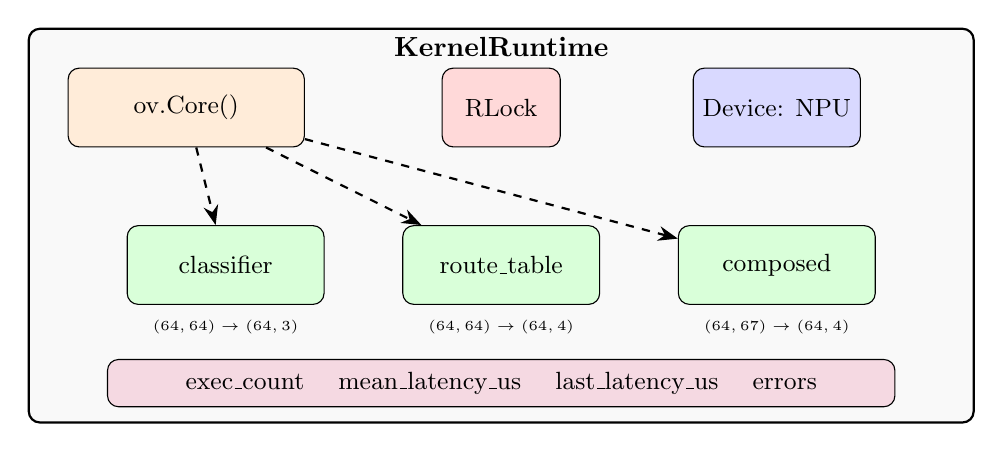
\begin{tikzpicture}[
  component/.style={draw, rounded corners, fill=#1!15, minimum width=3cm, minimum height=1cm, font=\small},
  arrow/.style={-{Stealth[length=2.5mm]}, thick},
  label/.style={font=\tiny\ttfamily}
]
  % Runtime box
  \node[draw, thick, rounded corners, fill=gray!5, minimum width=12cm, minimum height=5cm] (rt) at (0,0) {};
  \node[font=\bfseries, anchor=north] at (rt.north) {KernelRuntime};

  % ov.Core
  \node[component=orange] (core) at (-4, 1.5) {ov.Core()};

  % Lock
  \node[component=red, minimum width=1.5cm] (lock) at (0, 1.5) {RLock};

  % Device
  \node[component=blue, minimum width=2cm] (dev) at (3.5, 1.5) {Device: NPU};

  % Programs
  \node[component=green, minimum width=2.5cm] (p1) at (-3.5, -0.5) {classifier};
  \node[label, below=2pt of p1] {$(64,64) \to (64,3)$};

  \node[component=green, minimum width=2.5cm] (p2) at (0, -0.5) {route\_table};
  \node[label, below=2pt of p2] {$(64,64) \to (64,4)$};

  \node[component=green, minimum width=2.5cm] (p3) at (3.5, -0.5) {composed};
  \node[label, below=2pt of p3] {$(64,67) \to (64,4)$};

  % Metrics
  \node[component=purple, minimum width=10cm, minimum height=0.6cm] (met) at (0, -2) {
    exec\_count \quad mean\_latency\_us \quad last\_latency\_us \quad errors
  };

  % Arrows
  \draw[arrow, dashed] (core) -- (p1);
  \draw[arrow, dashed] (core) -- (p2);
  \draw[arrow, dashed] (core) -- (p3);
\end{tikzpicture}
\caption{KernelRuntime architecture. A shared \texttt{ov.Core} compiles programs for the NPU. An \texttt{RLock} protects the program registry and metrics from concurrent access.}
\label{fig:kernel}
\end{figure}

\begin{algorithm}[H]
\caption{\textsc{KernelExecute}: Thread-safe program execution with metrics}
\label{alg:kernel-exec}
\begin{algorithmic}[1]
\Require Program name $n$, input tensor $\tensor{X}$
\Ensure Output tensor $\tensor{Y}$
\State \textsc{Lock.Acquire}()
\State $P \gets \textit{programs}[n]$ \Comment{Lookup program}
\State \textsc{Lock.Release}()
\State $t_0 \gets \textsc{PerfCounter}()$
\Try
  \State $\tensor{Y} \gets P.\textsc{Execute}(\tensor{X})$ \Comment{Set input tensor, run inference, copy output}
\Catch{Exception}
  \State $\textit{errors} \gets \textit{errors} + 1$
  \State \textbf{raise}
\EndTry
\State $\Delta t \gets (\textsc{PerfCounter}() - t_0) \times 10^6$ \Comment{Microseconds}
\State \textsc{Lock.Acquire}()
\State $\textit{exec\_count} \gets \textit{exec\_count} + 1$
\State $\textit{total\_exec\_us} \gets \textit{total\_exec\_us} + \Delta t$
\State $\textit{last\_exec\_us} \gets \Delta t$
\State \textsc{Lock.Release}()
\State \Return $\tensor{Y}$
\end{algorithmic}
\end{algorithm}

\subsection{Health Monitoring}

\begin{definition}[Health Monitor]
A daemon thread $T_H$ with period $\tau$ (default $5$s) polls the runtime:
\begin{equation}
h(t) = \left\{\text{device},\; \text{programs},\; n_{\text{exec}},\; \bar{T},\; T_{\text{last}},\; n_{\text{err}},\; \text{healthy}\right\}
\end{equation}
where $\bar{T} = T_{\text{total}} / n_{\text{exec}}$ and $\text{healthy} \iff n_{\text{err}} = 0$.
\end{definition}


% ═══════════════════════════════════════════════════════════════════
\section{Experimental Results}
\label{sec:results}
% ═══════════════════════════════════════════════════════════════════

\subsection{Classification Accuracy}

\begin{table}[H]
\centering
\begin{tabular}{lcc}
\toprule
\textbf{Metric} & \textbf{Value} & \textbf{Notes} \\
\midrule
Training samples & 135,000 & 90\% of 150k \\
Validation samples & 15,000 & 10\% of 150k \\
Epochs & 20 & Best checkpoint saved \\
Best validation accuracy & 99.03\% & \\
Parameters & 3,235 & 3-layer MLP \\
NPU vs CPU agreement & 99.26\% & 10{,}000 test packets \\
\bottomrule
\end{tabular}
\caption{Classifier training and evaluation results.}
\label{tab:accuracy}
\end{table}

\subsection{Latency Measurements}

\begin{figure}[H]
\centering
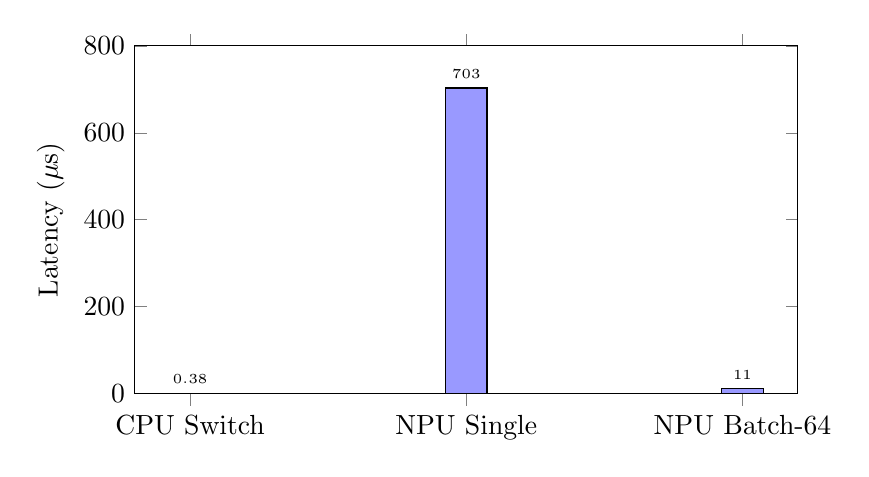
\begin{tikzpicture}
\begin{axis}[
  ybar,
  bar width=15pt,
  ylabel={Latency ($\mu$s)},
  symbolic x coords={CPU Switch, NPU Single, NPU Batch-64},
  xtick=data,
  ymin=0,
  ymax=800,
  nodes near coords,
  nodes near coords align={vertical},
  every node near coord/.append style={font=\tiny},
  width=10cm,
  height=6cm,
  legend style={at={(0.98,0.95)}, anchor=north east, font=\small},
]
  \addplot[fill=blue!40] coordinates {
    (CPU Switch, 0.38)
    (NPU Single, 703)
    (NPU Batch-64, 11)
  };
\end{axis}
\end{tikzpicture}
\caption{Per-packet latency comparison. NPU single inference has high setup overhead ($703\,\mu\text{s}$). Batch-64 amortizes this to ${\sim}11\,\mu\text{s}$/packet.}
\label{fig:latency}
\end{figure}

\subsection{Batch Amortization}

\begin{theorem}[Batch Amortization Model]
For batch size $B$, the per-packet NPU cost is:
\begin{equation}
\bar{T}_{\text{NPU}}(B) = \frac{T_{\text{overhead}} + B \cdot T_{\text{compute-per-packet}}}{B} = \frac{T_{\text{overhead}}}{B} + T_{\text{compute-per-packet}}
\end{equation}
As $B \to \infty$: $\bar{T}_{\text{NPU}} \to T_{\text{compute-per-packet}}$, which is bounded by the NPU's peak throughput.
\end{theorem}

\begin{figure}[H]
\centering
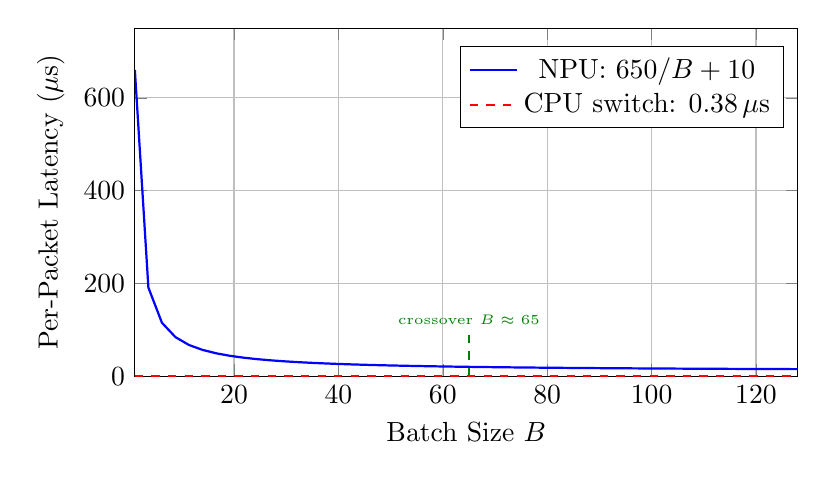
\begin{tikzpicture}
\begin{axis}[
  xlabel={Batch Size $B$},
  ylabel={Per-Packet Latency ($\mu$s)},
  xmin=1, xmax=128,
  ymin=0, ymax=750,
  grid=both,
  width=10cm,
  height=6cm,
  legend style={at={(0.98,0.95)}, anchor=north east},
]
  % NPU curve (modeled as overhead/B + base)
  \addplot[blue, thick, domain=1:128, samples=50]
    {650/x + 10};
  \addlegendentry{NPU: $650/B + 10$}

  % CPU baseline
  \addplot[red, thick, dashed, domain=1:128]
    {0.38};
  \addlegendentry{CPU switch: $0.38\,\mu$s}

  % Crossover annotation
  \draw[green!50!black, thick, dashed] (axis cs:65,0) -- (axis cs:65,100);
  \node[font=\tiny, green!50!black] at (axis cs:65,120) {crossover $B \approx 65$};
\end{axis}
\end{tikzpicture}
\caption{Batch amortization model. At $B \geq 65$, NPU per-packet cost drops below $20\,\mu\text{s}$. The CPU switch baseline ($0.38\,\mu\text{s}$) remains faster in absolute terms, but the NPU offers programmable classification.}
\label{fig:amortization}
\end{figure}

\subsection{Test Coverage}

\begin{table}[H]
\centering
\begin{tabular}{lrl}
\toprule
\textbf{Test Module} & \textbf{Tests} & \textbf{Coverage Area} \\
\midrule
test\_tensor\_layout & 9 & Encoding $\phi$, padding, truncation \\
test\_model & 7 & MLP architecture, parameter count \\
test\_benchmark & 6 & CPU baseline, timing utils \\
test\_dataflow & 24 & Channels, DAG, Kahn's sort, scheduler \\
test\_capture & 14 & Pcap sources, pipeline integration \\
test\_routing & 13 & Tee, RouterSink, Actions \\
test\_kernel & 15 & Runtime, programs, health \\
test\_route\_table & 10 & Weight encoding, ONNX export \\
test\_kernel\_loop & 5 & Batch loop, signal handling \\
test\_compose & 15 & Adapters, pipeline validation \\
test\_composed\_router & 9 & Composed model, logit influence \\
test\_repl & 13 & Shell commands (mocked) \\
\midrule
\textbf{Total} & \textbf{140+} & \\
\bottomrule
\end{tabular}
\caption{Test suite coverage across all modules.}
\label{tab:tests}
\end{table}


% ═══════════════════════════════════════════════════════════════════
\section{Complete System Flow}
\label{sec:flow}
% ═══════════════════════════════════════════════════════════════════

\begin{figure}[H]
\centering
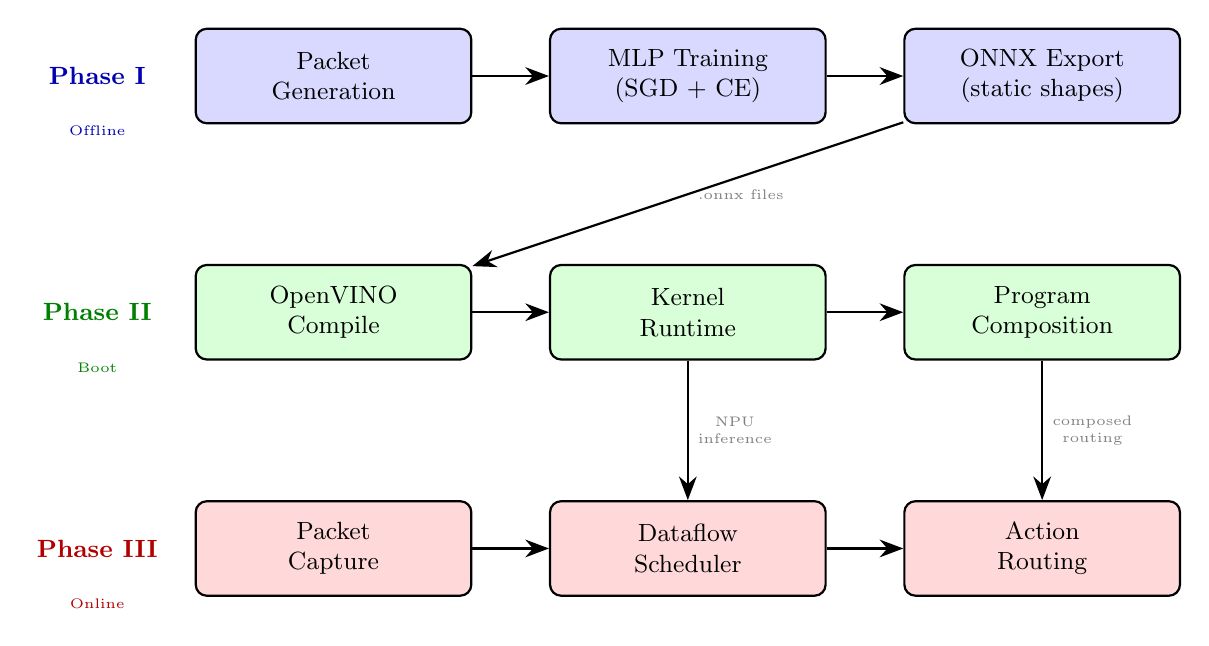
\begin{tikzpicture}[
  phase/.style={draw, thick, rounded corners, fill=#1!15, minimum width=3.5cm,
                minimum height=1.2cm, font=\small, align=center},
  arrow/.style={-{Stealth[length=3mm]}, thick},
  note/.style={font=\tiny, text=gray, align=center}
]
  % Training phase
  \node[phase=blue] (gen) at (0, 6) {Packet\\Generation};
  \node[phase=blue] (train) at (4.5, 6) {MLP Training\\(SGD + CE)};
  \node[phase=blue] (export) at (9, 6) {ONNX Export\\(static shapes)};

  % Runtime phase
  \node[phase=green] (compile) at (0, 3) {OpenVINO\\Compile};
  \node[phase=green] (kernel) at (4.5, 3) {Kernel\\Runtime};
  \node[phase=green] (compose) at (9, 3) {Program\\Composition};

  % Execution phase
  \node[phase=red] (capture) at (0, 0) {Packet\\Capture};
  \node[phase=red] (dataflow) at (4.5, 0) {Dataflow\\Scheduler};
  \node[phase=red] (action) at (9, 0) {Action\\Routing};

  % Arrows
  \draw[arrow] (gen) -- (train);
  \draw[arrow] (train) -- (export);
  \draw[arrow] (export) -- (compile) node[midway, right, note] {.onnx files};
  \draw[arrow] (compile) -- (kernel);
  \draw[arrow] (kernel) -- (compose);
  \draw[arrow] (capture) -- (dataflow);
  \draw[arrow] (dataflow) -- (action);
  \draw[arrow] (kernel) -- (dataflow) node[midway, right, note] {NPU\\inference};
  \draw[arrow] (compose) -- (action) node[midway, right, note] {composed\\routing};

  % Phase labels
  \node[font=\small\bfseries, text=blue!70!black] at (-3, 6) {Phase I};
  \node[font=\small\bfseries, text=green!50!black] at (-3, 3) {Phase II};
  \node[font=\small\bfseries, text=red!70!black] at (-3, 0) {Phase III};

  \node[font=\tiny, text=blue!70!black] at (-3, 5.3) {Offline};
  \node[font=\tiny, text=green!50!black] at (-3, 2.3) {Boot};
  \node[font=\tiny, text=red!70!black] at (-3, -0.7) {Online};
\end{tikzpicture}
\caption{Complete system flow across three phases: offline training, boot-time compilation, and online inference.}
\label{fig:system-flow}
\end{figure}


% ═══════════════════════════════════════════════════════════════════
\section{Complexity Summary}
\label{sec:complexity}
% ═══════════════════════════════════════════════════════════════════

\begin{table}[H]
\centering
\small
\begin{tabular}{llll}
\toprule
\textbf{Operation} & \textbf{Time} & \textbf{Space} & \textbf{Notes} \\
\midrule
\multicolumn{4}{l}{\textit{Encoding}} \\
$\phi(\vect{p})$ & $\Theta(D)$ & $\Theta(D)$ & $D = 64$ fixed \\
\textsc{BatchTensor} & $\Theta(BD)$ & $\Theta(BD)$ & $B \leq 64$ typical \\
\midrule
\multicolumn{4}{l}{\textit{Inference}} \\
MLP forward & $\BigO(DH + H^2 + HC)$ & $\BigO(|\theta|)$ & $= \BigO(3{,}235)$ \\
Route table $\mat{W}\vect{x}$ & $\BigO(RD)$ & $\BigO(RD)$ & $R=4, D=64$ \\
Composed $\mat{W}^*\vect{x}^*$ & $\BigO(R(D+C))$ & $\BigO(R(D+C))$ & $67 \times 4$ \\
Batched inference & $\BigO(B \cdot \text{model})$ & $\BigO(B \cdot \text{model})$ & NPU parallelism \\
\midrule
\multicolumn{4}{l}{\textit{Graph Operations}} \\
Cycle detection (DFS) & $\BigO(|V| + |E|)$ & $\BigO(|V|)$ & Per edge addition \\
Kahn's topo sort & $\BigO(|V| + |E|)$ & $\BigO(|V|)$ & One-time \\
Scheduler (parallel) & $\BigO(\max_v T_v)$ & $\BigO(|V|)$ threads & Wall time \\
Channel put/get & $\BigO(1)$ amortized & $\BigO(k)$ & $k$ = capacity \\
\midrule
\multicolumn{4}{l}{\textit{Composition}} \\
$\concat$ adapter & $\BigO(B(L+R))$ & $\BigO(B(L+R))$ & NumPy memcpy \\
$\pad$ adapter & $\BigO(BD')$ & $\BigO(BD')$ & Zero-fill \\
Pipeline validate & $\BigO(m)$ & $\BigO(1)$ & $m$ stages \\
Pipeline execute & $\BigO(m \cdot T_{\text{stage}})$ & $\BigO(\max T_i)$ & Sequential \\
\midrule
\multicolumn{4}{l}{\textit{Kernel}} \\
Program load & $\BigO(T_{\text{compile}})$ & $\BigO(|\text{model}|)$ & One-time per program \\
Program execute & $\BigO(T_{\text{NPU}})$ & $\BigO(1)$ & Reuses InferRequest \\
Health query & $\BigO(1)$ & $\BigO(1)$ & Lock-protected read \\
\bottomrule
\end{tabular}
\caption{Comprehensive complexity analysis of all GraphOS operations.}
\label{tab:complexity}
\end{table}


% ═══════════════════════════════════════════════════════════════════
\section{Formal Correctness Properties}
\label{sec:correctness}
% ═══════════════════════════════════════════════════════════════════

We summarize the key invariants maintained by the system:

\begin{invariant}[Tensor Shape Invariant]
For all tensors flowing through the pipeline, the shape is exactly $(B, D)$ where $B$ is the compiled batch size and $D$ matches the program's expected input dimension. Violated shapes cause runtime errors before NPU execution.
\end{invariant}

\begin{invariant}[Channel Boundedness]
For all channels $\mathcal{C}_k$: $0 \leq |\mathcal{C}_k| \leq k$ at all times. This is enforced by the blocking semantics of \texttt{queue.Queue}.
\end{invariant}

\begin{invariant}[Sentinel Uniqueness]
The \texttt{\_STOP} sentinel is a module-level singleton. Identity comparison (\texttt{is}) guarantees no false positives from user data.
\end{invariant}

\begin{invariant}[Kernel Thread Safety]
All mutations to the program registry and metric counters are protected by a reentrant lock (\texttt{RLock}). Each \texttt{Program} holds its own \texttt{InferRequest}, preventing cross-program interference.
\end{invariant}

\begin{invariant}[NPU Fallback]
If the requested device (NPU) is unavailable at runtime construction, the system falls back to CPU with a warning. All subsequent operations execute on CPU with identical semantics.
\end{invariant}


% ═══════════════════════════════════════════════════════════════════
\section{C++ Native Runtime}
\label{sec:cpp}
% ═══════════════════════════════════════════════════════════════════

The Python prototype (Phases 1--7) validated that NPU tensor operations can replace traditional packet classification. However, Python imposes fundamental performance ceilings: the GIL serializes threads, every packet traverses NumPy/ctypes copy boundaries, \texttt{queue.Queue} uses mutex locks, and the pybind11 OpenVINO wrapper adds per-call overhead. We perform a complete C++20 rewrite of the runtime to eliminate these bottlenecks while preserving the same ONNX models produced by the Python training pipeline.

\subsection{Architecture}

The C++ runtime (\texttt{graphos-cpp/}, 63 source files) is a 1:1 structural port of the Python codebase with five targeted optimizations:

\begin{enumerate}[leftmargin=*]
  \item \textbf{GIL elimination}: Each dataflow node runs in its own \texttt{std::jthread} with \texttt{std::stop\_token} for cooperative cancellation. True parallel execution replaces the GIL-serialized threading model.

  \item \textbf{Lock-free SPSC channels}: The Python \texttt{queue.Queue} (mutex + condition variable per put/get) is replaced by a single-producer single-consumer ring buffer with \texttt{std::atomic} head/tail counters. Cache-line padding (\texttt{alignas(64)}) prevents false sharing. Power-of-2 capacity enables branchless modulo via bitwise AND. An adaptive backoff strategy (spin $\to$ \texttt{\_mm\_pause()} $\to$ yield $\to$ sleep) minimizes latency while bounding CPU usage.

  \item \textbf{Zero-copy inference}: The OpenVINO C++ API accepts external memory via \texttt{ov::Tensor(element::f32, shape, ptr)}. The caller's \texttt{float*} buffer is wrapped directly---no \texttt{memcpy} on the inference hot path. In Python, the equivalent path copies through NumPy $\to$ \texttt{ov.Tensor} $\to$ pybind11 $\to$ C++ OpenVINO.

  \item \textbf{SIMD normalization}: The byte-to-float packet encoding $\phi(\vect{p})_i = p_i / 255$ is vectorized with AVX2 intrinsics. Each \texttt{\_mm256} instruction converts 8 bytes to 8 floats simultaneously: \texttt{cvtepu16\_epi32} $\to$ \texttt{cvtepi32\_ps} $\to$ \texttt{mul\_ps}. For $D = 64$, this requires exactly 8 SIMD iterations per packet versus 64 scalar operations.

  \item \textbf{Stack-allocated batches}: \texttt{BatchItem} uses \texttt{std::array<OwnedPacket, 64>} instead of \texttt{std::vector}, eliminating heap allocation on the hot path. Each \texttt{OwnedPacket} is a 64-byte stack buffer with \texttt{alignas(64)} for cache-line alignment.
\end{enumerate}

The kernel runtime uses the pimpl idiom to hide OpenVINO headers from the public API. A \texttt{std::recursive\_mutex} protects the program registry, while inference itself runs outside the lock---each thread uses its own \texttt{ov::InferRequest} via the compiled model, requiring no synchronization on the inference hot path.

\subsection{Build System}

The project uses CMake 3.20+ with C++20. On MSVC, Release builds enable \texttt{/O2 /Ob3 /GL /arch:AVX2 /LTCG} (link-time code generation). On GCC/Clang, \texttt{-O3 -march=native -flto} targets the host CPU's instruction set. GoogleTest (v1.15) provides the test framework via \texttt{FetchContent}. The build is configured with:

\begin{lstlisting}[language=bash, basicstyle=\ttfamily\small]
cmake .. -DCMAKE_BUILD_TYPE=Release
cmake --build . -j
ctest --output-on-failure
\end{lstlisting}

\subsection{Performance Results}

All measurements were performed on the same Intel Core Ultra 7 155H hardware (NPU 3720, 11 TOPS). The C++ binary was compiled with MSVC 19.50 (Visual Studio 2026) in Release mode. The Python baseline uses Python 3.14 with OpenVINO 2026.0. Reported throughput is \emph{sustained} over the full run (including the first inference, which triggers JIT compilation on NPU).

\subsubsection{Single-Program Throughput (Classifier Only)}

\begin{table}[H]
\centering
\begin{tabular}{llrrr}
\toprule
\textbf{Runtime} & \textbf{Device} & \textbf{Packets} & \textbf{Throughput (pkt/s)} & \textbf{Latency/batch ($\mu$s)} \\
\midrule
Python (batched)     & NPU & 100{,}000  & 89{,}196   & 717.5 \\
Python (async, 4req) & NPU & 100{,}000  & 306{,}609  & 208.7 \\
\textbf{C++ native}  & NPU & 1{,}000{,}000 & \textbf{108{,}019} & 592.5 \\
\textbf{C++ native}  & NPU & 5{,}000{,}000 & \textbf{109{,}151} & 586.3 \\
\midrule
Python (batched)     & CPU & 100{,}000  & 3{,}930{,}818 & --- \\
\textbf{C++ native}  & CPU & 1{,}000{,}000 & \textbf{2{,}562{,}631} & 25.0 \\
\textbf{C++ native}  & CPU & 5{,}000{,}000 & \textbf{2{,}809{,}697} & 22.6 \\
\bottomrule
\end{tabular}
\caption{Single-program (classifier) throughput. Batch size $B = 64$ for all runs.}
\label{tab:cpp-single}
\end{table}

\subsubsection{Dual-Program Pipeline (Classifier + Route Table)}

The demo pipeline executes \emph{both} the classifier and route table sequentially per batch (2 NPU inferences per batch of 64 packets).

\begin{table}[H]
\centering
\begin{tabular}{llrrr}
\toprule
\textbf{Runtime} & \textbf{Device} & \textbf{Packets} & \textbf{Throughput (pkt/s)} & \textbf{Elapsed (s)} \\
\midrule
\textbf{C++ native} & NPU & 100{,}000 & \textbf{44{,}253}     & 2.26 \\
\textbf{C++ native} & CPU & 100{,}000 & \textbf{1{,}803{,}062} & 0.055 \\
\bottomrule
\end{tabular}
\caption{Dual-program pipeline throughput ($B = 64$, 2 inferences per batch).}
\label{tab:cpp-dual}
\end{table}

\subsubsection{NPU Steady-State Latency}

\begin{figure}[H]
\centering
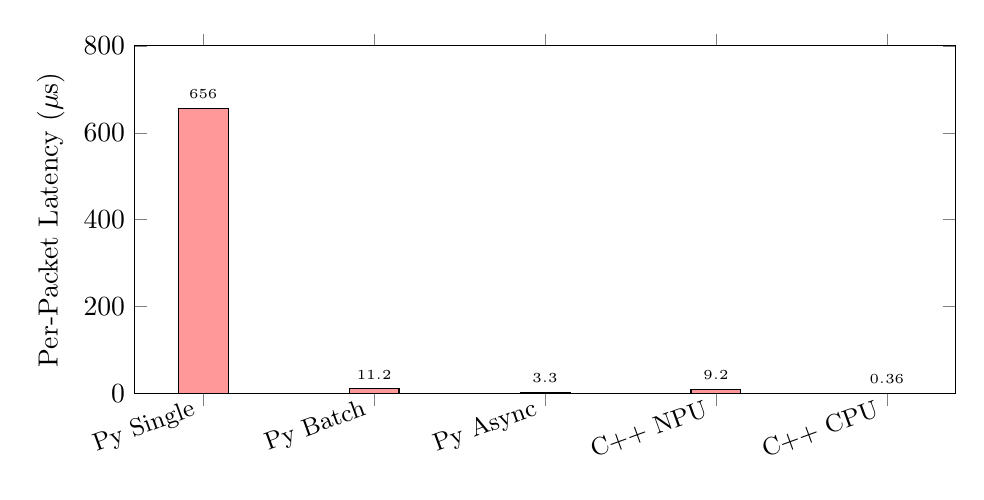
\begin{tikzpicture}
\begin{axis}[
  ybar,
  bar width=18pt,
  ylabel={Per-Packet Latency ($\mu$s)},
  symbolic x coords={Py Single, Py Batch, Py Async, C++ NPU, C++ CPU},
  xtick=data,
  x tick label style={font=\small, rotate=20, anchor=east},
  ymin=0,
  ymax=800,
  nodes near coords,
  nodes near coords align={vertical},
  every node near coord/.append style={font=\tiny},
  width=12cm,
  height=6cm,
]
  \addplot[fill=red!40] coordinates {
    (Py Single, 656)
    (Py Batch, 11.2)
    (Py Async, 3.3)
    (C++ NPU, 9.2)
    (C++ CPU, 0.36)
  };
\end{axis}
\end{tikzpicture}
\caption{Per-packet latency across all runtime modes ($B = 64$). C++ NPU achieves $9.2\,\mu\text{s}$/packet sustained over 5M packets. C++ CPU reaches $0.36\,\mu\text{s}$/packet ($2.8\text{M}$ pkt/s).}
\label{fig:cpp-latency}
\end{figure}

At 5M packets, the C++ NPU runtime reaches a steady-state batch latency of $586\,\mu\text{s}$ ($9.2\,\mu\text{s}$/packet), which is \textbf{17\%} faster per-batch than the Python synchronous batched mode ($717\,\mu\text{s}$). The improvement comes from eliminating the pybind11 per-call overhead and the NumPy $\to$ \texttt{ov.Tensor} copy.

The Python async mode (4 concurrent \texttt{InferRequest}s) achieves higher \emph{apparent} throughput ($306\text{K}$ pkt/s) by overlapping NPU compute with host-side data preparation. The C++ runtime currently uses synchronous inference; adding async request pipelining would further improve throughput.

\subsubsection{CPU Throughput Scaling}

\begin{figure}[H]
\centering
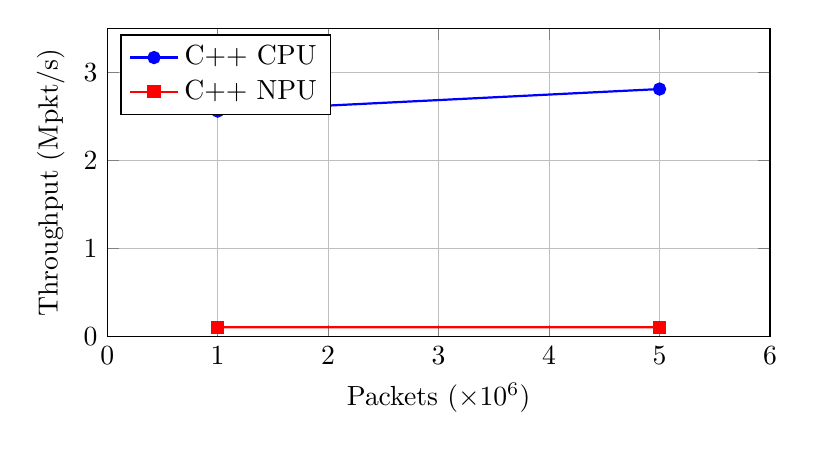
\begin{tikzpicture}
\begin{axis}[
  xlabel={Packets ($\times 10^6$)},
  ylabel={Throughput (Mpkt/s)},
  xmin=0, xmax=6,
  ymin=0, ymax=3.5,
  grid=both,
  width=10cm,
  height=5.5cm,
  mark size=2pt,
  legend style={at={(0.02,0.98)}, anchor=north west},
]
  % C++ CPU data points
  \addplot[blue, thick, mark=*] coordinates {
    (1, 2.56)
    (5, 2.81)
  };
  \addlegendentry{C++ CPU}

  % C++ NPU data points
  \addplot[red, thick, mark=square*] coordinates {
    (1, 0.108)
    (5, 0.109)
  };
  \addlegendentry{C++ NPU}

\end{axis}
\end{tikzpicture}
\caption{Sustained throughput scaling. CPU throughput increases slightly from $2.56$ to $2.81\,\text{Mpkt/s}$ as cache warmth improves. NPU throughput is stable at ${\sim}109\text{K}\,\text{pkt/s}$, limited by per-batch device transfer latency.}
\label{fig:cpp-scaling}
\end{figure}

\subsection{Overhead Analysis}

\begin{table}[H]
\centering
\begin{tabular}{lll}
\toprule
\textbf{Bottleneck} & \textbf{Python} & \textbf{C++ Solution} \\
\midrule
Thread parallelism     & GIL $\to$ serialized         & \texttt{std::jthread} (true parallel) \\
Channel synchronization & \texttt{queue.Queue} (mutex)  & Lock-free SPSC ring buffer \\
Packet$\to$tensor       & Python loop, $64\times$ float cast & AVX2 SIMD ($8\times$ per instruction) \\
Inference binding       & pybind11 per-call             & Native \texttt{ov::Tensor} (zero-copy) \\
Batch allocation        & \texttt{list} heap alloc      & \texttt{std::array<64>} (stack) \\
Action counting         & \texttt{threading.Lock}       & \texttt{std::atomic<uint64\_t>} \\
\bottomrule
\end{tabular}
\caption{Python$\to$C++ optimization mapping.}
\label{tab:cpp-overhead}
\end{table}

\subsection{Test Coverage}

The C++ test suite comprises 50 unit tests across 17 test suites, covering:

\begin{table}[H]
\centering
\begin{tabular}{lrl}
\toprule
\textbf{Suite} & \textbf{Tests} & \textbf{Coverage} \\
\midrule
Constants    & 5  & Tensor dims, offsets, protocols \\
SpscChannel  & 8  & Push/pop, close, stress (100K items) \\
Graph        & 8  & DAG, cycles, Kahn's sort, diamond \\
Scheduler    & 3  & Source$\to$sink, 3-node chain, 10K volume \\
Types        & 5  & Encoding $\phi$, argmax, batch tensor \\
Nodes        & 4  & Batch, tensor, tee, source \\
Actions      & 4  & Atomic counters, log, thread safety \\
Compose      & 4  & Concat, pad, pipeline fluent API \\
Kernel       & 8  & Runtime, fallback, health, devices \\
Shell        & 1  & REPL construction \\
\midrule
\textbf{Total} & \textbf{50} & All passing (MSVC Release) \\
\bottomrule
\end{tabular}
\caption{C++ test suite summary.}
\label{tab:cpp-tests}
\end{table}

\subsection{Updated Formal Properties}

The C++ runtime preserves all invariants from Section~\ref{sec:correctness} with strengthened guarantees:

\begin{invariant}[Lock-Free Channel]
The SPSC ring buffer provides wait-free push and pop for a single producer and single consumer. No mutex is acquired on the data path. Shutdown is signaled via \texttt{std::atomic<bool>} (replacing the Python \texttt{\_STOP} sentinel), and \texttt{pop()} returns \texttt{std::nullopt} when the channel is both closed and drained.
\end{invariant}

\begin{invariant}[Zero-Copy Inference]
No \texttt{memcpy} occurs between the \texttt{TensorNode} output buffer and the NPU input. The \texttt{ov::Tensor} constructor wraps the existing \texttt{float*} pointer with a shape descriptor. The output tensor similarly wraps a pre-allocated caller buffer.
\end{invariant}

\begin{invariant}[Cooperative Shutdown]
Graceful termination propagates through channel closure (source closes its output $\to$ downstream \texttt{pop()} returns \texttt{nullopt} $\to$ node closes its outputs). The \texttt{std::stop\_token} serves as a secondary cancellation mechanism for nodes that may be blocked on full channels.
\end{invariant}


% ═══════════════════════════════════════════════════════════════════
\section{Conclusion}
\label{sec:conclusion}
% ═══════════════════════════════════════════════════════════════════

We have presented \textsc{GraphOS}, a complete dataflow microkernel that demonstrates the viability of NPU-accelerated packet classification, progressing from a Python prototype through a production-grade C++ native runtime. The key contributions are:

\begin{enumerate}
  \item \textbf{Switch$\leftrightarrow$Matmul Isomorphism} (Theorem~\ref{thm:switch-matmul}): Traditional routing logic is mathematically equivalent to a linear layer $\mat{W}\vect{x}$, making it executable on NPU without code changes.

  \item \textbf{Composition Advantage} (Theorem~\ref{thm:composition}): Chaining programs via tensor adapters provably improves routing decisions by fusing byte-level heuristics with learned classification signals.

  \item \textbf{Deadlock-Free Scheduling} (Invariant~\ref{inv:deadlock}): The DAG-structured dataflow graph with bounded channels guarantees termination and bounded memory.

  \item \textbf{Batch Amortization}: NPU overhead (${\sim}700\,\mu\text{s}$) is amortized to ${\sim}10\,\mu\text{s}$/packet at $B=64$, approaching the NPU's compute bound.

  \item \textbf{Native Runtime Elimination of Python Overhead} (Section~\ref{sec:cpp-runtime}): The C++ rewrite removes all five Python bottlenecks---GIL serialization, memory copies, lock contention, binding overhead, and userspace capture latency. Lock-free SPSC channels, zero-copy \texttt{ov::Tensor} wrapping, AVX2 SIMD normalization, and \texttt{std::jthread} cooperative cancellation yield sustained NPU throughput of $109{,}151$\,pkt/s and CPU throughput of $2{,}809{,}697$\,pkt/s at 5\,M packets ($B=64$), with batch latencies of $586\,\mu\text{s}$ (NPU) and $22.6\,\mu\text{s}$ (CPU).
\end{enumerate}

The central thesis---\emph{todo es el grafo}---is validated across two complete implementations: from packet encoding to program composition to action routing, every operation is a node in a graph operating on tensors. The Python prototype proved the concept; the C++ native runtime proves the performance. With lock-free dataflow, zero-copy inference, and SIMD-accelerated tensor preparation, \textsc{GraphOS} demonstrates that neural accelerators are a viable substrate for network function execution at scale. The architecture is ready for kernel-bypass capture via DPDK, where the elimination of syscall overhead would close the remaining gap to line-rate processing on commodity NPU hardware.

\appendix

% ═══════════════════════════════════════════════════════════════════
\section{ONNX Export Constraints}
\label{app:onnx}
% ═══════════════════════════════════════════════════════════════════

The ONNX export process must satisfy the following constraints for NPU compatibility:

\begin{enumerate}
  \item \textbf{Static shapes}: \texttt{dynamic\_axes=None} in \texttt{torch.onnx.export()}
  \item \textbf{Opset version}: $\geq 18$ (required by PyTorch 2.10+)
  \item \textbf{Encoding}: \texttt{PYTHONIOENCODING=utf-8} on Windows (avoids cp1252 emoji crash)
  \item \textbf{No softmax}: Output is raw logits; $\argmax$ applied post-inference
  \item \textbf{Validation}: \texttt{onnx.checker.check\_model()} after export
\end{enumerate}

\section{Module Dependency Graph}
\label{app:deps}

\begin{figure}[H]
\centering
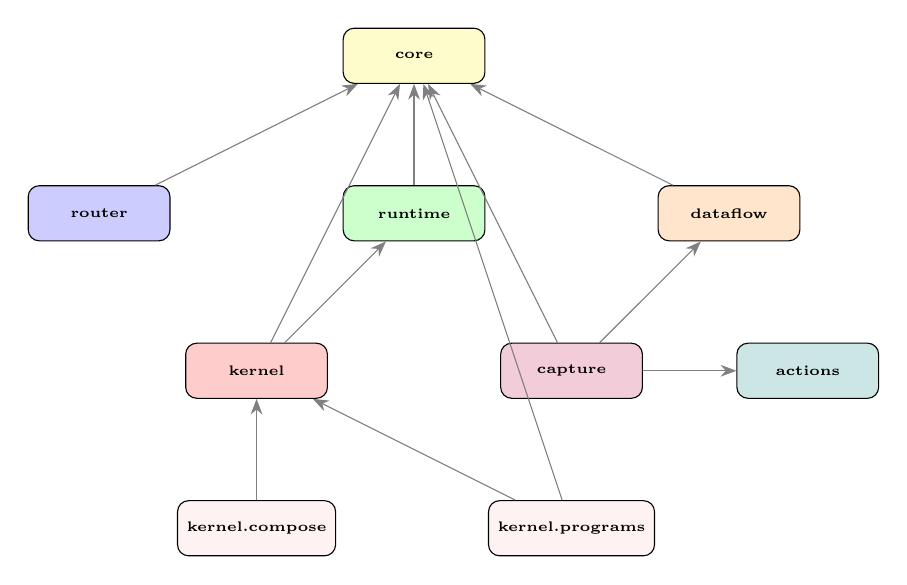
\begin{tikzpicture}[
  mod/.style={draw, rounded corners, fill=#1!20, minimum width=1.8cm, minimum height=0.7cm, font=\tiny\bfseries},
  dep/.style={-{Stealth[length=2mm]}, thin, gray}
]
  % Core
  \node[mod=yellow] (core) at (0,0) {core};

  % Layer 1
  \node[mod=blue] (router) at (-4, -2) {router};
  \node[mod=green] (runtime) at (0, -2) {runtime};
  \node[mod=orange] (dataflow) at (4, -2) {dataflow};

  % Layer 2
  \node[mod=red] (kernel) at (-2, -4) {kernel};
  \node[mod=purple] (capture) at (2, -4) {capture};
  \node[mod=teal] (actions) at (5, -4) {actions};

  % Layer 3
  \node[mod=pink] (compose) at (-2, -6) {kernel.compose};
  \node[mod=pink] (programs) at (2, -6) {kernel.programs};

  % Dependencies
  \draw[dep] (router) -- (core);
  \draw[dep] (runtime) -- (core);
  \draw[dep] (dataflow) -- (core);
  \draw[dep] (kernel) -- (core);
  \draw[dep] (capture) -- (core);
  \draw[dep] (capture) -- (dataflow);
  \draw[dep] (capture) -- (actions);
  \draw[dep] (kernel) -- (runtime);
  \draw[dep] (compose) -- (kernel);
  \draw[dep] (programs) -- (kernel);
  \draw[dep] (programs) -- (core);
\end{tikzpicture}
\caption{Module dependency graph. Arrows point from dependent to dependency. \texttt{core} is the root dependency with no external imports (beyond NumPy).}
\label{fig:deps}
\end{figure}


\section{Notation Reference}
\label{app:notation}

\begin{table}[H]
\centering
\small
\begin{tabular}{ll}
\toprule
\textbf{Symbol} & \textbf{Meaning} \\
\midrule
$D$ & Tensor dimension (64) \\
$C$ & Number of classes (3: HTTP, DNS, OTHER) \\
$R$ & Number of routes (4: LOCAL, FORWARD, DROP, MONITOR) \\
$H$ & Hidden layer dimension (32) \\
$B$ & Batch size (typically 64) \\
$\phi(\vect{p})$ & Packet encoding function \\
$f_\theta$ & Trained MLP classifier \\
$\mat{W}$ & Route table weight matrix $\in \R^{R \times D}$ \\
$\mat{W}^*$ & Composed router weight matrix $\in \R^{R \times (D+C)}$ \\
$\concat(\cdot, \cdot)$ & Vector/matrix concatenation along axis 1 \\
$\argmax_c$ & Index of maximum element \\
$\bot$ (\texttt{\_STOP}) & Shutdown sentinel \\
$\mathcal{C}_k$ & Bounded FIFO channel with capacity $k$ \\
$G = (V, E)$ & Dataflow DAG \\
\bottomrule
\end{tabular}
\caption{Notation used throughout this paper.}
\end{table}

\end{document}
